% Header
\renewcommand\evenpagerightmark{{\scshape\small Chapter 4}}
\renewcommand\oddpageleftmark{{\scshape\small Amplification processes in gaseous detectors}}

\renewcommand{\bibname}{References}

\hyphenation{}

\chapter[Physics of Resistive plate chambers]%
{Physics of Resistive plate chambers}
\label{chapt4}

A \acf{RPC} is a gaseous detector used in high-energy physics experiments as described in Chapter~\ref{chapt:3}. It has been developed in 1981 by Santonico and Cardarelli~\cite{SANTONICO81}, under the name of \textit{Resistive Plate Counter}, as an alternative to the local-discharge spark counters proposed in 1978 by Pestov and Fedotovich~\cite{PESTOV78,FEDOTOVICH82}. Working with spark chambers implied using high-pressure gas and high mechanical precision which the RPC simplified by formerly using a gas mixture of argon and butane flowed at atmospheric pressure and a constant and uniform electric field propagated in between two parallel electrode plates. Moreover, a significant increase in rate capability was introduced by the use of electrode plate material with high bulk resistivity, preventing the discharge from growing throughout the whole gas gap. Indeed, the effect of using resistive electrodes is that the constant electric field is locally canceled out by the development of the discharge, limiting its growth.
	
	Through its development history, different operating modes~\cite{CROTTY93,CROTTY94,CARDARELLI96}, gas mixtures~\cite{SANTONICO81,CARDARELLI93,CARDARELLI96,ABBRESCIA1997PERF,ABBRESCIA1997,CAMARRI98,ZEBALLOS98} and new detector designs~\cite{ZEBALLOS96MRPC,WILLIAMS98,CZYRKOWSKI98} have been discovered, leading to further improvement of the rate capability of such a detector. The low developing costs and easily achievable large detection areas offered by RPCs, as well as the wide range of possible designs, made them a natural choice to as muon chambers and/or trigger detectors in multipurpose experiments such as CMS~\cite{MUONTDR} or ATLAS~\cite{ATLASTDR}, time-of-flight detectors in ALICE~\cite{ALICETDR}, calorimeter with CALICE~\cite{CALICE2016} or even detectors for volcanic muography with ToMuVol~\cite{TOMUVOL2011}. 

\section{Principle}
\label{chapt4:sec:principle}

	RPCs are ionisation detectors composed of two parallel resistive plate electrodes in between which a constant electric field is set. The space in between the electrodes, referred to as \textit{gap}, is filled with a dense gas that is used to generate primary ionization into the gas volume. The free charge carriers (electrons and cations) created by the ionization of the gas molecules are then accelerated towards the electrodes by the electric field, as shown in Figure~\ref{fig:RPC_principle}~\cite{LIPPMANN2003}. RPCs being passive detectors, a current on pick-up copper read-out placed outside of the gas volume is induced by the charge accumulation during the growth of the avalanche resulting from the acceleration of the charge carriers. As a consequence, the time resolution of the detector is substantially increased as the output signal is generated while the electrons are still in movement. The advantage of a constant electric field, over multi-wire proportional chambers, is that the electrons are being fully accelerated from the moment charge carriers are freed and feel the full strength of the electric field that doesn't depend on the distance to the readout and that the output signal doesn't need for the electrons to be physically collected.
	
	\begin{figure}[H]
		\centering
		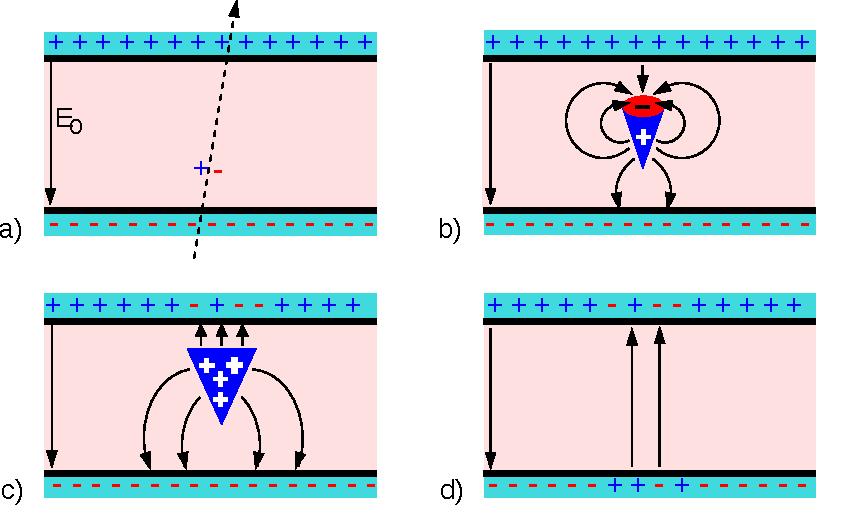
\includegraphics[width = \plotwidth]{fig/chapt4/RPC_principle.pdf}\\
		\caption{\label{fig:RPC_principle} Different phases of the avalanche development in the RPC gas volume subjected to a constant electric field $E_0$. a) An avalanche is initiated by the primary ionisation caused by the passage of a charged particle through the gas volume. b) Due to its growing size, the avalanche starts to locally influence the electric field. c) The electrons, lighter than the cations reach the anode first. d) The ions reach the cathode. While the charges have not recombined, the electric field in the small region around the avalanche stays affected and locally blinds the detector.}
	\end{figure}
	
	After an avalanche developed in the gas, a time long compared to the development of a discharge is needed to recombine the charge carriers in the electrode material due to their resistivity. This property has the advantage of affecting the local electric field and avoiding sparks in the detector but, on the other hand, the rate capability is intrinsically limited by the time constant $\tau_{RPC}$ of the detector. Using a quasi-static approximation of Maxwell’s equations for weakly conducting media, it can be shown that the time constant $\tau_{RPC}$ necessary to the charge recombination at the interface in between the electrode and the gas volume is given by the Formula~\ref{for:tau}~\cite{RIEGLER2002}.
	
	\begin{equation}
		\label{for:tau}
		\tau_{RPC} = \frac{\epsilon_{electrode}+\epsilon_{gas}}{\sigma_{electrode}+\sigma_{gas}}
	\end{equation}
	
	A gas can be assimilated to vacuum, leading to $\epsilon_{gas} = \epsilon_0$ and $\sigma_{gas} = 0$, and the electrodes permittivity and conductivity can be written as $\epsilon_{electrode} = \epsilon_r\epsilon_0$ and $\sigma_{electrode} = 1/\rho_{electrode}$, showing the strong dependence of the time constant to the electrodes resistivity in Formula~\ref{for:taurho}.
	
	\begin{equation}
		\label{for:taurho}
		\tau_{RPC} = (\epsilon_r + 1)\epsilon_0\times\rho_{electrode}
	\end{equation}
	
	Very few materials with a low enough resistivity exist in nature. The resistivity targeted to build RPCs ranges from $10^9$ to $10^{12}$ \si{\ohm\cdot cm}. The most common RPC electrode materials are displayed in Table~\ref{tab:tau}. When the doped glass and ceramics can offer short time constants of the order of \SI{1}{ms}, the developing cost of such materials is quite high due to the very low demand. Thus, \acf{HPL} is often the choice for high rate experiments using very large RPC detection areas. Other experiments working at cosmic muon fluxes can safely operate with ordinary float glass.
	
	\begin{table}[H]
		\centering
		\begin{tabular}{|l|c|c|c|}
		\hline
		Material & $\rho_{electrode}$ (\si{\ohm\cdot cm}) & $\epsilon_r$ & $\tau_{RPC}$ (\si{ms})\\
		\hline
		Float glass & $10^{12}$ & $\sim$7 & $\sim$700\\
		\acl{HPL} & $10^{10}$ to $10^{12}$ & $\sim$6 & $\sim$6 to 600\\
		Doped glass (LR S) & $10^{9}$ to $10^{11}$ & $\sim$10 & $\sim$1 to 100\\
		Doped ceramics (SiN/SiC) & $10^{9}$ & $\sim$8.5 & $\sim$1\\
		Doped ceramics (Ferrite) & $10^{8}$ to $10^{12}$ & $\sim$20 & $\sim$0.2 to 2000\\
		\hline
		\end{tabular}
		\caption{\label{tab:tau} Properties of the most used electrode materials for RPCs.}
	\end{table}

\section{Rate capability and time resolution of Resistive Plate Chambers}
\label{chapt4:sec:RateCapa}

	The electrode material plays a key role in the maximum intrinsic rate capability of RPCs. R\&D is continuously being done to develop at always cheaper costs material with lower resistivity. Nevertheless, the amount of charge released, i.e. the size of the discharge, if reduced leads to a smaller blind area in the detector, increasing the rate capability of the detector. On the other hand, the drift velocity of electrons in the gas volume being quite stable with the applied electric field, the design of a detector and the associated read-out and pulse-processing electronics will be a major component of the time resolution of RPCs. Moreover, the sensitivity of the electronics will also help increasing the rate capability by lowering the gain the gas volume needs to be operated at, increasingly lowering the gas volume in which the signals will develop.
	
	\subsection{Operation modes}
	\label{chapt4:ssec:operation}
	
	Being a gaseous detector using an accelerating electric field to amplify the signal of primary charge carriers, the RPC can be operated into different modes as the electric field intensity varies. Each mode offers different performances for such a detector, and it will be showed that the operating mode corresponding to the lowest electric field possible is best suited for high rate detectors working in collider experiments.
	
	RPCs where developed early 1980s. At that time it was using an operating mode now referred to as \textit{streamer mode}. Streamers are large discharges that develop in between the 2 electrodes enough to locally discharge the electrodes. If the electric field inside of the gas volume is strong enough, with electrons being fast compared to ions, a large and dense cloud of positive ions will develop nearby the anode and extend toward the cathode while the electrons are being collected, eventually leading to a streamer discharge due to the increase of field seen at the cathode. The field is then strong enough so that electrons are pulled out of the cathode. Electrodes, though they are a unique volume of resistive material, can be assimilated to capacitors. At the moment an electric field is applied in between their outer surfaces, the charge carriers inside of the volume will start moving leading to a situation where there is no voltage across the electrodes and a higher density of negative charges, i.e. electrons, on the inner surface of the cathode. Finally, when a streamer discharge occurs, these electrons are partially released in the gas volume contributing to increase the discharge strength until the formation of a conductive plasma, the streamer. This can be understood through Figure~\ref{fig:ElecCharge}~\cite{CROTTY93}. Streamer signals are very convenient in terms of read-out as no further amplification is required with output pulses amplitudes of the order of a few tens to few hundreds of \si{mV} as can be seen on Figure~\ref{fig:ModeSignal}.
	
	\begin{figure}[H]
		\begin{subfigure}{0.5\linewidth}
			\centering
			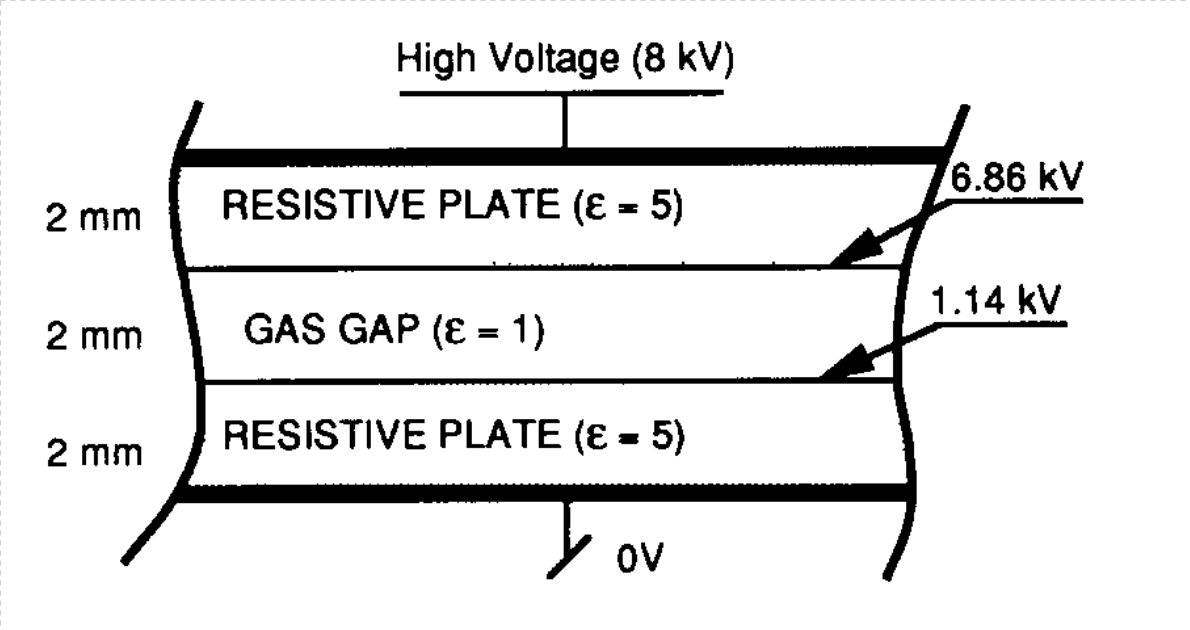
\includegraphics[width = 0.5\plotwidth]{fig/chapt4/RPC_Charging_1.png}
			\caption{\label{fig:ElecCharge:A}}
		\end{subfigure}
		\begin{subfigure}{0.5\linewidth}
			\centering
			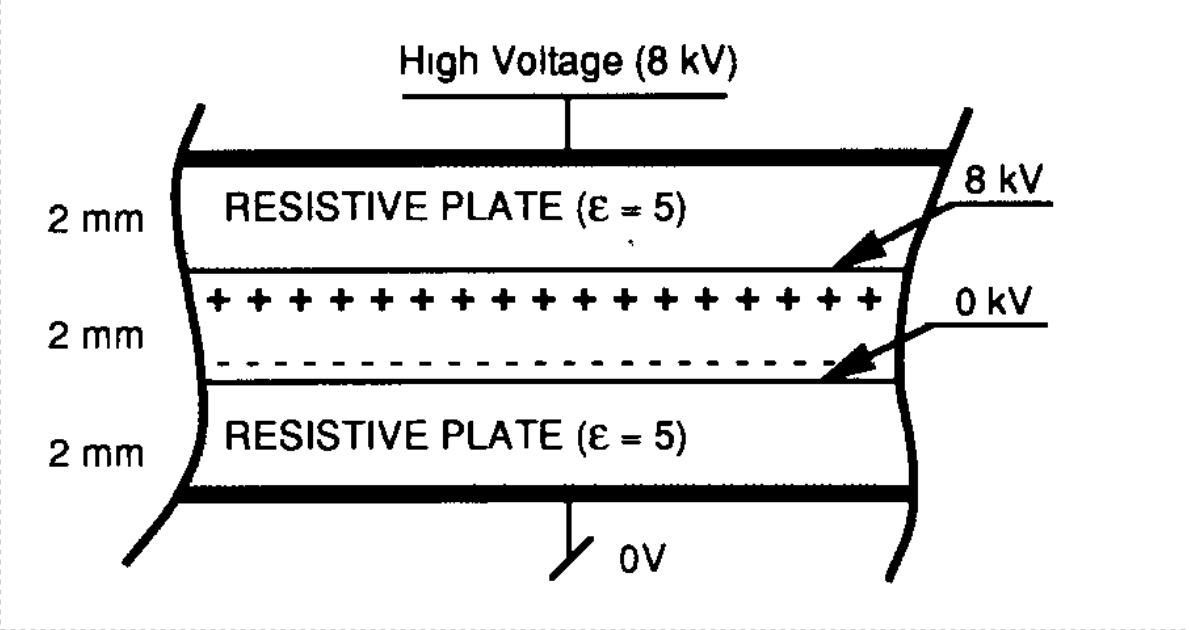
\includegraphics[width = 0.5\plotwidth]{fig/chapt4/RPC_Charging_2.png}\\
			\caption{\label{fig:ElecCharge:B}}
		\end{subfigure}
		\begin{subfigure}{\linewidth}
			\centering
			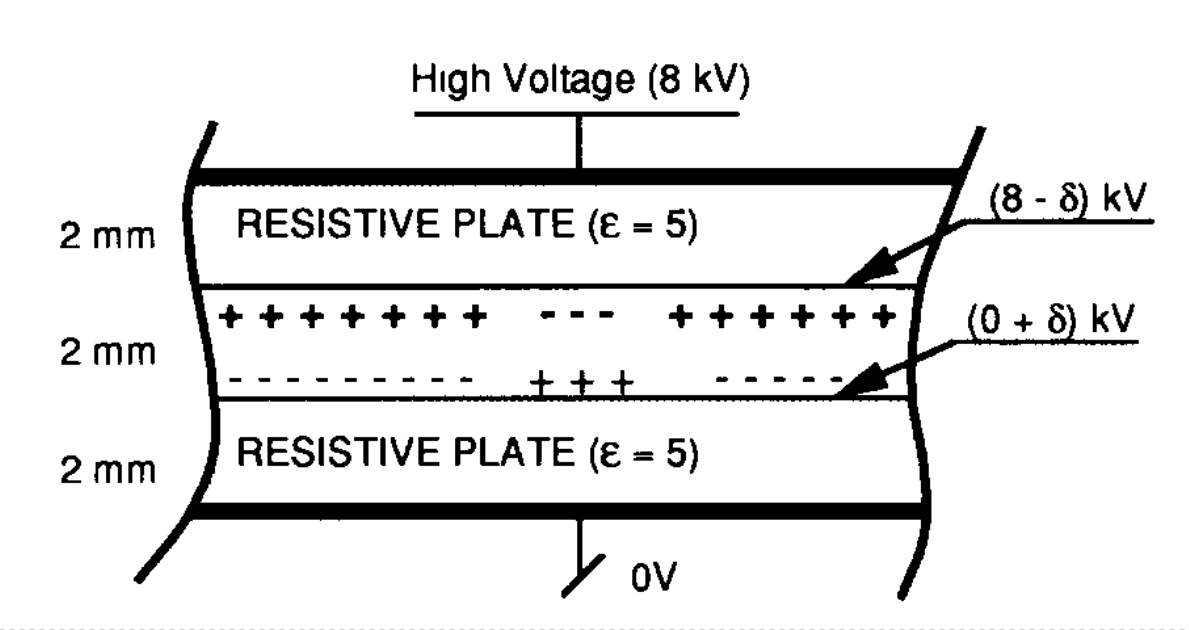
\includegraphics[width = 0.5\plotwidth]{fig/chapt4/RPC_Charging_3.png}
			\caption{\label{fig:ElecCharge:C}}
		\end{subfigure}
		\caption{\label{fig:ElecCharge} Movement of the charge carriers in an RPC. Figure~\ref{fig:ElecCharge:A}: Voltage across an RPC whose electrode have a relative permittivity of 5 at the moment the tension s applied. Figure~\ref{fig:ElecCharge:B}: After the charge carriers moved, the electrodes are charged and there is no voltage drop over the electrodes anymore. The full potential is applied on the gas gap only. Figure~\ref{fig:ElecCharge:C}: The streamer discharge initiated by a charged particle transports electrons and cations towards the anode and cathode respectively.}
	\end{figure}
	
	\begin{figure}[H]
		\begin{subfigure}{0.5\linewidth}
			\centering
			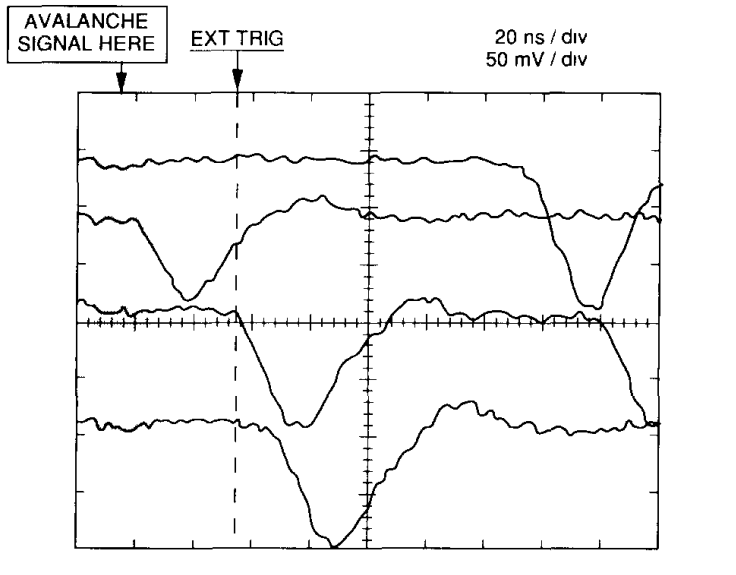
\includegraphics[width = 0.5\plotwidth]{fig/chapt4/RPC_Streamer_Mode.png}
			\caption{\label{fig:ModeSignal:A}}
		\end{subfigure}
		\begin{subfigure}{0.5\linewidth}
			\centering
			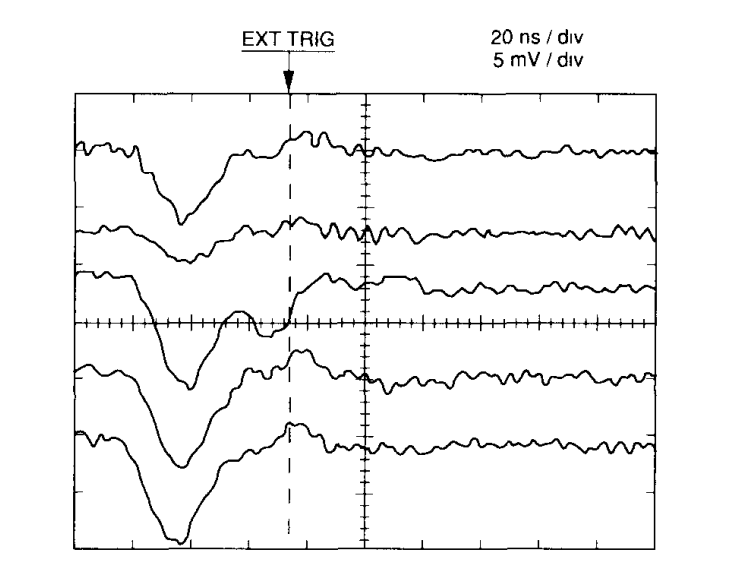
\includegraphics[width = 0.5\plotwidth]{fig/chapt4/RPC_Avalanche_Mode.png}\\
			\caption{\label{fig:ModeSignal:B}}
		\end{subfigure}
		\caption{\label{fig:ModeSignal} Typical oscilloscope pulses in streamer mode (Figure~\ref{fig:ModeSignal:A}) and avalanche mode(Figure~\ref{fig:ModeSignal:B}). In the case of streamer mode, the very small avalanche signal is visible.}
	\end{figure}
	
	When the electric field is reduced though, the electronic gain is small until the electrons get close enough to the anode and the positive ion cloud is much smaller. The electric field cannot rise to the point a field emission of electrons on the cathode is possible. The resulting signal is weak, of the order of a few \si{mv} as shown on Figure~\ref{fig:ModeSignal}, and requires amplification. This is the \textit{avalanche mode} of RPC operation. This mode offers a higher rate capability by providing smaller discharges that don't affect the electrodes charge and are more locally contained in the gas volume as was demonstrated by Crotty with Figure~\ref{fig:ModeRate}~\cite{CROTTY93}. The detector only stays locally blind the time the charge carriers are recombined and there is no need for electrode recharge which is a long process affecting a large portion of the detector. Another advantage of avalanche signals over streamer is the great time consistency. Figure~\ref{fig:ModeSignal} shows very clearly that avalanche signals have a very small time jitter. Thus, using such a mode is a natural choice for experiments in which the detectors are required to have a high detection rate.
	
	\begin{figure}[H]
		\centering
		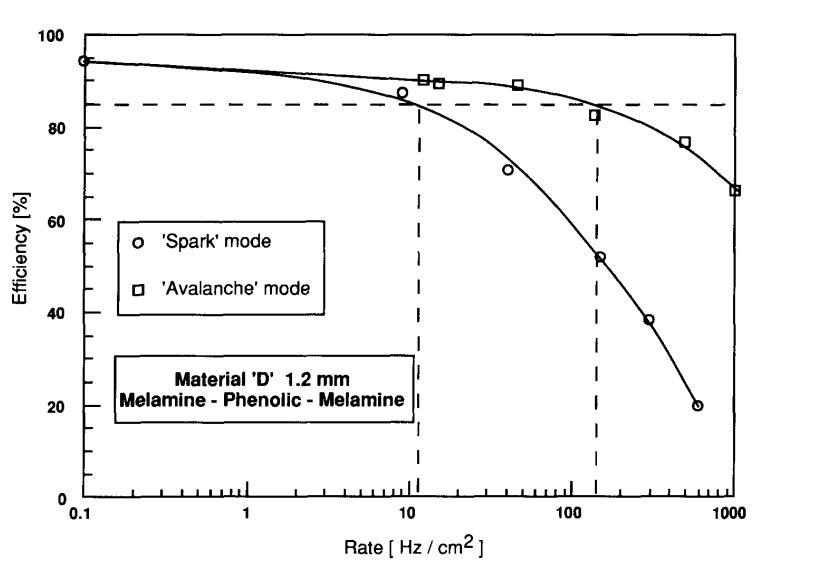
\includegraphics[width = \plotwidth]{fig/chapt4/Rate_Mode_Comparison.png}
		\caption{\label{fig:ModeRate} Rate capability comparison for the streamer and avalanche mode of operation. An order of magnitude in rate capability for a maximal efficiency drop of 10\% is gained by using the avalanche mode over the streamer mode.}
	\end{figure}

	\subsection{Standard gas mixture for RPCs operated in collider experiments}
	\label{chat4:ssec:gasmix}
	
	The first RPC working in streamer mode was operated with a 50/50 mixture of argon and butane~\cite{SANTONICO81}, a standard mixture used at that time in multi-wire proportional chambers, taking profit of the good effective Townsend coefficient of argon to maximize the number of primary charge carriers freed in the gas by ionizing particles and of the quenching properties of butane. Before the discovery of the avalanche mode of RPC operation and concerned about the rate capability of RPCs operated in streamer mode, the performance improvement of the detectors through the increase of fast charge ratio in the signal development ,decreasing the charge induced per avalanche as can be seen through Figure~\ref{fig:FreonCharge}, was studied by adding Freon based gases, such as $CF_3Br$, into the typical $Ar$/$C_4H_{10}$ gas mixture was studied and showed that a lower induced charge could lead to an improvement the rate capability~\cite{CARDARELLI93}. This consideration lead to the discovery of the avalanche mode which confirmed that the smaller the induced charge, the better the rate capability of the RPCs~\cite{CROTTY93}. This discovery could happen thanks to the increased number of lower induced charge events allowed by adding a fraction of strong quencher in the gas mixture.
	
	\begin{figure}[H]
		\begin{subfigure}{0.5\linewidth}
			\centering
			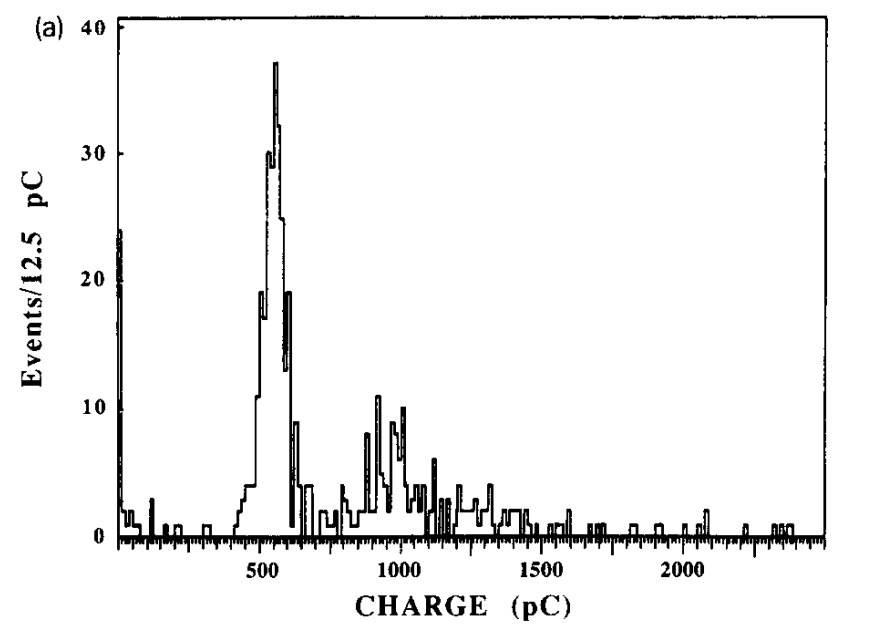
\includegraphics[width = 0.5\plotwidth]{fig/chapt4/Gas-mix-0-freon.png}
			\caption{\label{fig:FreonCharge:A}}
		\end{subfigure}
		\begin{subfigure}{0.5\linewidth}
			\centering
			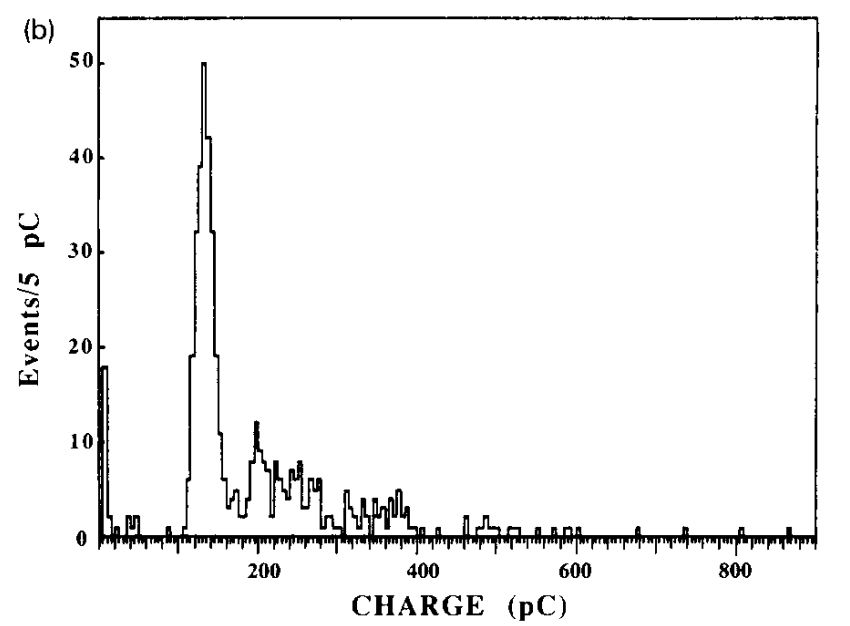
\includegraphics[width = 0.5\plotwidth]{fig/chapt4/Gas-mix-4-freon.png}
			\caption{\label{fig:FreonCharge:B}}
		\end{subfigure}
		\begin{subfigure}{\linewidth}
			\centering
			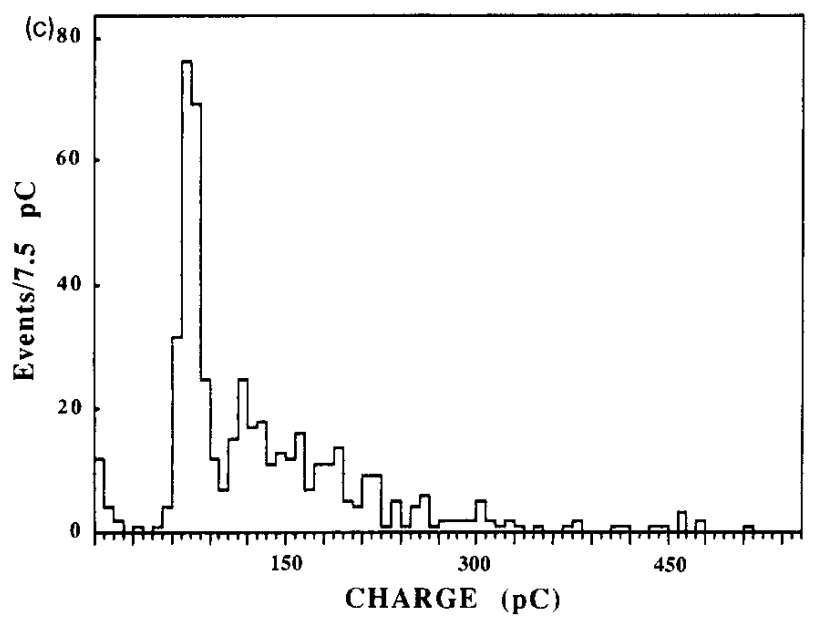
\includegraphics[width = 0.5\plotwidth]{fig/chapt4/Gas-mix-8-freon.png}\\
			\caption{\label{fig:FreonCharge:C}}
		\end{subfigure}
		\caption{\label{fig:FreonCharge} Comparison of the charge distribution of signals induced by cosmic muons in an RPC operated with a gas mixture of argon, butane and bromotrifluoromethane ($CF_3Br$). The $Ar$/$C_4H_10$ is kept constant at 60/40 in volume while the total amount of $CF_3Br$ in the mixture is varied: 0\% (Figure~\ref{fig:FreonCharge:A}), 4\% (Figure~\ref{fig:FreonCharge:B}) and 8\% (Figure~\ref{fig:FreonCharge:C})~\cite{CARDARELLI93}.}
	\end{figure}
	
	\begin{figure}[H]
		\begin{subfigure}{0.5\linewidth}
			\centering
			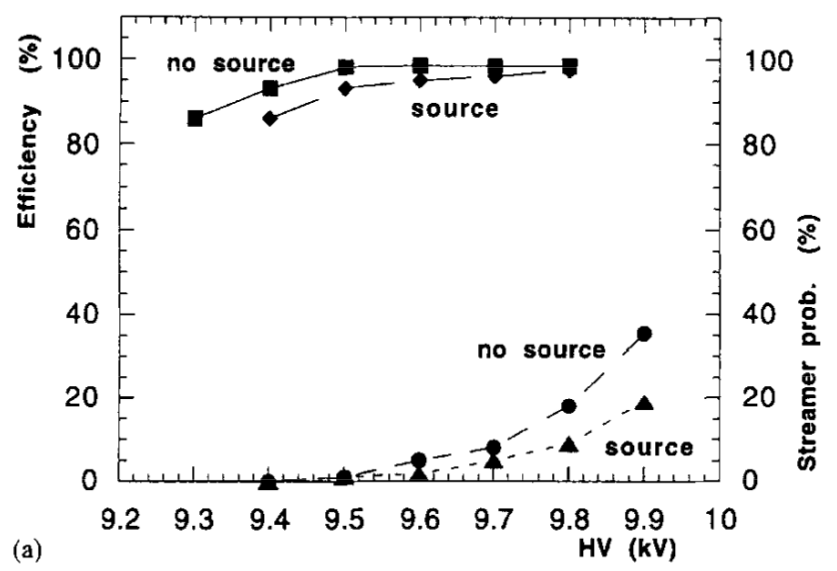
\includegraphics[width = 0.5\plotwidth]{fig/chapt4/Freon-perf-irrad.png}
			\caption{\label{fig:FreonArgonPerf:A}}
		\end{subfigure}
		\begin{subfigure}{0.5\linewidth}
			\centering
			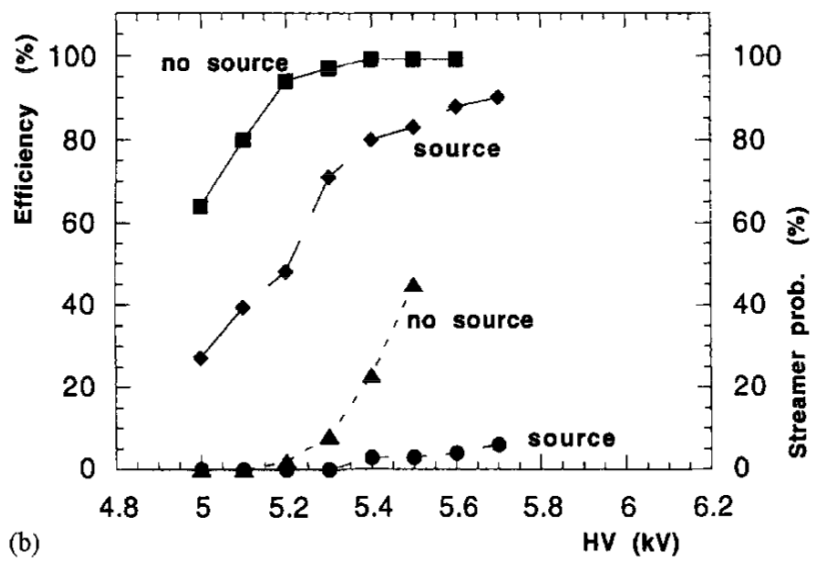
\includegraphics[width = 0.5\plotwidth]{fig/chapt4/Argon-perf-irrad.png}
			\caption{\label{fig:FreonArgonPerf:B}}
		\end{subfigure}
		\caption{\label{fig:FreonArgonPerf} Comparison of the efficiency and streamer probability, defined as the fraction of events with an induced charge 10 times larger than that of the average avalanche, with and without irradiation by a \SI{24}{GBq} $^{137}Cs$ source of an RPC successively operated with a 90/10 mixture $C_2H_2F_4$/i-$C_4H_{10}$ (Figure~\ref{fig:FreonArgonPerf:A}) and a 70/5/10/15 mixture of $Ar$/i-$C_4H_{10}$/$CO_2$/$C_2H_2F_4$ (Figure~\ref{fig:FreonArgonPerf:B})~\cite{ABBRESCIA1997PERF}.}
	\end{figure}
	
	From this moment onward, more and more studies were conducted in order to find a gas mixture that would allow for the best suppression of streamers for the benefit of low charge avalanches. Most R\&D groups working with narrow gaps started using freon-based gas mixtures while users of wide gap RPCs kept using $Ar$/$CO_2$ based mixtures. The differences in between narrow and wide gaps will be later discussed in Section~\ref{chapt4:ssec:design}. The $CF_3Br$ having a high GWP, tetrafluoroethane ($C_2H_2F_4$) was preferred to it as more suitable ecofriendly gas in the middle of the 90s. An advantage of this new freon component is that it featured a high primary ionization and a low operating voltage, as reported by Cardarelli~\cite{CARDARELLI96}. Thus, the new gas mixtures used were mainly composed of tetrafluoroethane alone with lower content of isobutane in order to reduce the flammability of the mixtures in the case it were to be used in accelerator experiments for safety reasons. Performance and models about such mixtures were discussed in papers of Abbrescia~\cite{ABBRESCIA1997PERF,ABBRESCIA1997} and showed a better suitability of such a gas mixture, with respect to argon based ones, for operations with high radiation backgrounds leading to a need for high rate capability of the detectors, as can be seen from Figures~\ref{fig:FreonArgonPerf} and \ref{fig:FreonArgonFastCharge}. Indeed, although the operating voltage of a tetrafluoroethane based mixture is higher than which of an argon based mixture but the efficiency under irradiation is more stable, the voltage range with negligible streamer probability is much wider, and the fast charge ratio available is much greater, providing with more stable operation of the detector.
	
	\begin{figure}[H]
		\begin{subfigure}{0.5\linewidth}
			\centering
			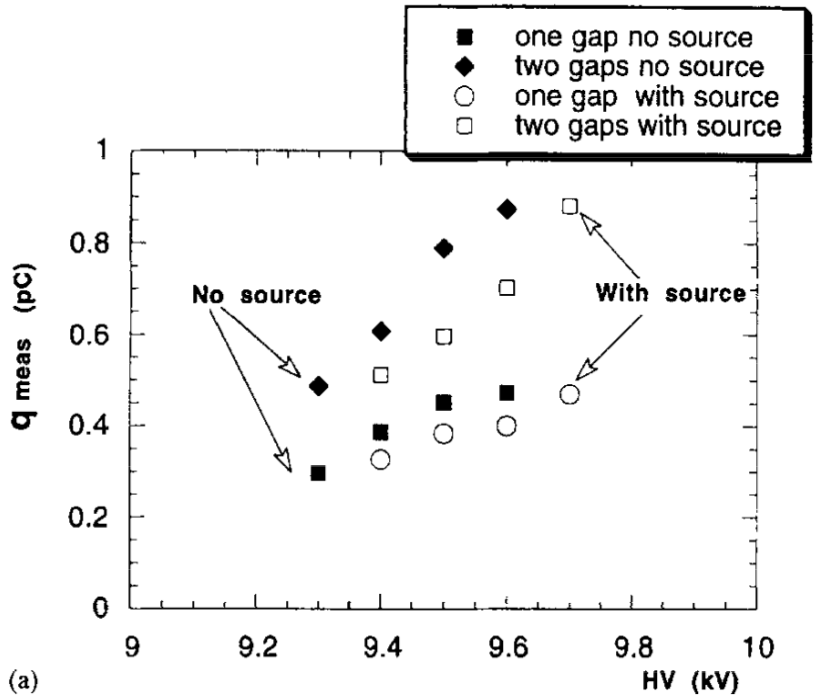
\includegraphics[width = 0.5\plotwidth]{fig/chapt4/Freon-fast-charge-irrad.png}
			\caption{\label{fig:FreonArgonFastCharge:A}}
		\end{subfigure}
		\begin{subfigure}{0.5\linewidth}
			\centering
			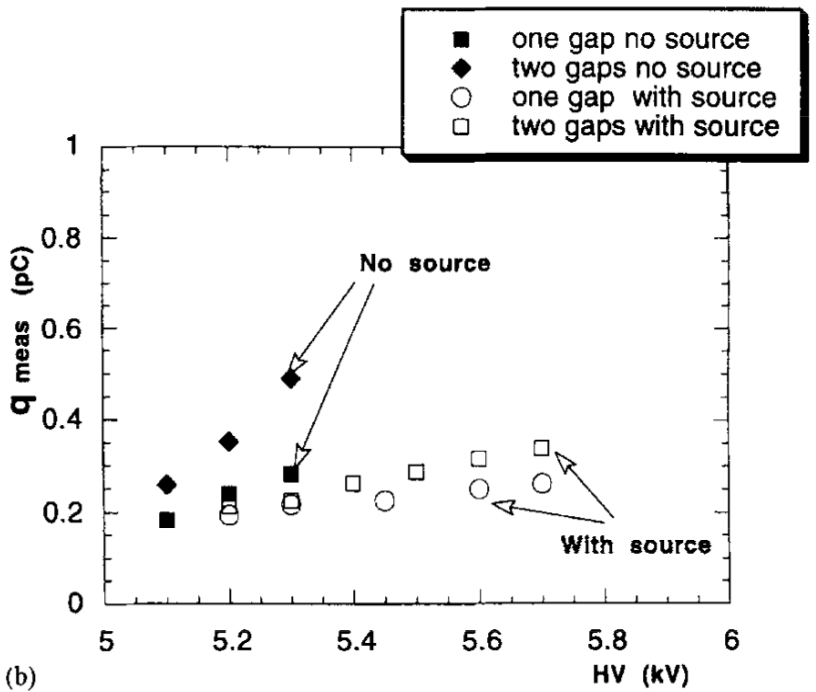
\includegraphics[width = 0.5\plotwidth]{fig/chapt4/Argon-fast-charge-irrad.png}
			\caption{\label{fig:FreonArgonFastCharge:B}}
		\end{subfigure}
		\caption{\label{fig:FreonArgonFastCharge} Comparison of the fast charge ratio with and without irradiation by a \SI{24}{GBq} $^{137}Cs$ source of an RPC successively operated with a 90/10 mixture $C_2H_2F_4$/i-$C_4H_{10}$ (Figure~\ref{fig:FreonArgonFastCharge:A}) and a 70/5/10/15 mixture of $Ar$/i-$C_4H_{10}$/$CO_2$/$C_2H_2F_4$ (Figure~\ref{fig:FreonArgonFastCharge:B}). The results are provided for both single gap and double gap operation~\cite{ABBRESCIA1997PERF}.}
	\end{figure}
	
	Aside of the improvement of the rate capability through linseed oil surface treatment of HPL electrodes, which allowed for a lower intrinsic noise rate and dark current of the detectors by improving the smoothness of the electrodes surface~\cite{ABBRESCIA1997OIL}, it was later found that the streamers could be further suppressed by adding an electronegative compound into the gas mixture. The benefits of adding $SF_6$ in order to push the transitions from avalanche to streamers towards high voltages has been discussed in 1998~\cite{CAMARRI98,ZEBALLOS98} and eventually the high rate RPC destined to be used in accelerator physics would unanimously start using this compound into RPC gas mixtures. Being able to control the creation of streamers allows for slower ageing of the detector and lower power consumption as the currents driven by the electrodes consecutively to the induced charges would be smaller. In summary, the typical gas mixture RPCs are operated with is generally composed of the following 3 gas compounds, although, as mentioned in Chapter~\ref{chapt3:sec:EcoGas}, research is being conducted into new more ecofriendly gas mixture using gases with a much lower \acl{GWP}:
	
	\begin{itemize}
		\item[•] Tetrafluoroethane ($C_2F_4H_2$), also referred to as \textit{Freon} or \textit{R134a}, is the principal compound of the RPC gas mixtures, with a typical fraction above 90\%. It is used for it's high effective Townsend coefficient and the great average fast charge that allows to operate the detector with a high threshold with respect to argon, for example, that has similar effective Townsend coefficient but suffers from a lower fast charge. To operate with similar conditions, argon would require a higher electric field leading to a higher fraction of streamers, thus limiting the rate capability of the detector~\cite{ABBRESCIA1997,ABBRESCIA1997PERF}.
		\item[•] Isobutane (i-$C_4H_{10}$), only present in a few percent in the gas mixtures, is used for its UV quenching properties~\cite{BATTISTONI85} helping to prevent streamers due to UV photon emission during the avalanche growth.
		\item[•] Sulfur hexafluoride, ($SF_6$), simply referred to as \textit{SF6}, is used in very little quantities for its high electronegativity. Excess of electrons are being absorbed by the compound and streamers are suppressed~\cite{CAMARRI98,ZEBALLOS98}. Nevertheless, a fraction of $SF_6$ higher than 1\% will not bring any extra benefice in terms of streamer cancelation power but will lead to higher operating voltage~\cite{CAMARRI98}, as can be understood through Figure~\ref{fig:SF6}.
	\end{itemize}
	
	\begin{figure}[H]
		\centering
		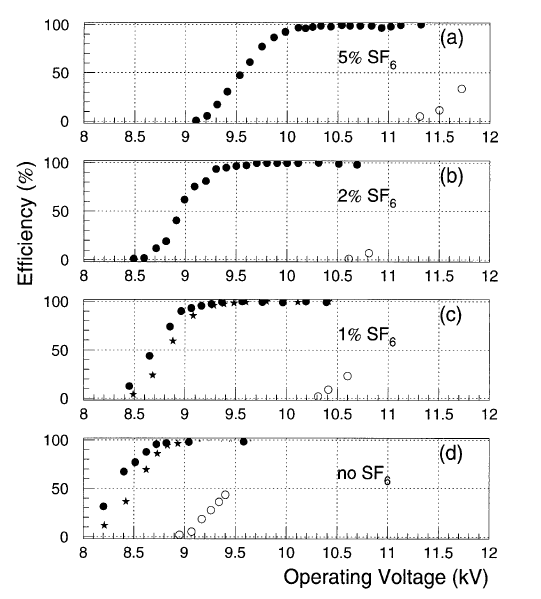
\includegraphics[width = 0.7\plotwidth]{fig/chapt4/SF6.png}
		\caption{\label{fig:SF6} Effeciency (circles and stars with \SI{30}{mV} and \SI{100}{mV} thresholds respectively) and streamer probability (opened circles) as function of the operating voltatge of a \SI{2}{mm} single gap HPL RPC flushed with a gas mixture containing (a) 5\%, (b) 2\%, (c) 1\% and (d) no $SF_6$~\cite{CAMARRI98}.}
	\end{figure}
	
	In the last steps of R\&D, the gas mixture of CMS RPCs was forseen to be a 96.2/3.5/0.3 composition of $C_2H_2F_4$/i-$C_4H_{10}$/$SF_6$~\cite{ABBRESCIA2005} but finally it was slightly changed into a 95.2/4.5/0.3 mixture of the same gases~\cite{THYSSEN2012}. A summary of the operation performance of the RPCs since the start of LHC and of CMS data taking is given in Figure~\ref{fig:CMSRPCperf}~\cite{SHAH2018}. The performance of the detectors is regularly monitored and the operating voltages updated in order to obtain a very stable performance through time. Nevertheless, the detectors will face new challenges during Phase-II during which they will exposed to more extreme radiation conditions. Description of the longevity tests with extreme irradiation and the conclusions regarding the operation of the present RPC system will be given in Chapter~\ref{chapt5}.
	
	\begin{figure}[H]
		\hspace*{-0.05\plotwidth}
		\begin{subfigure}{0.5\linewidth}
			\centering
			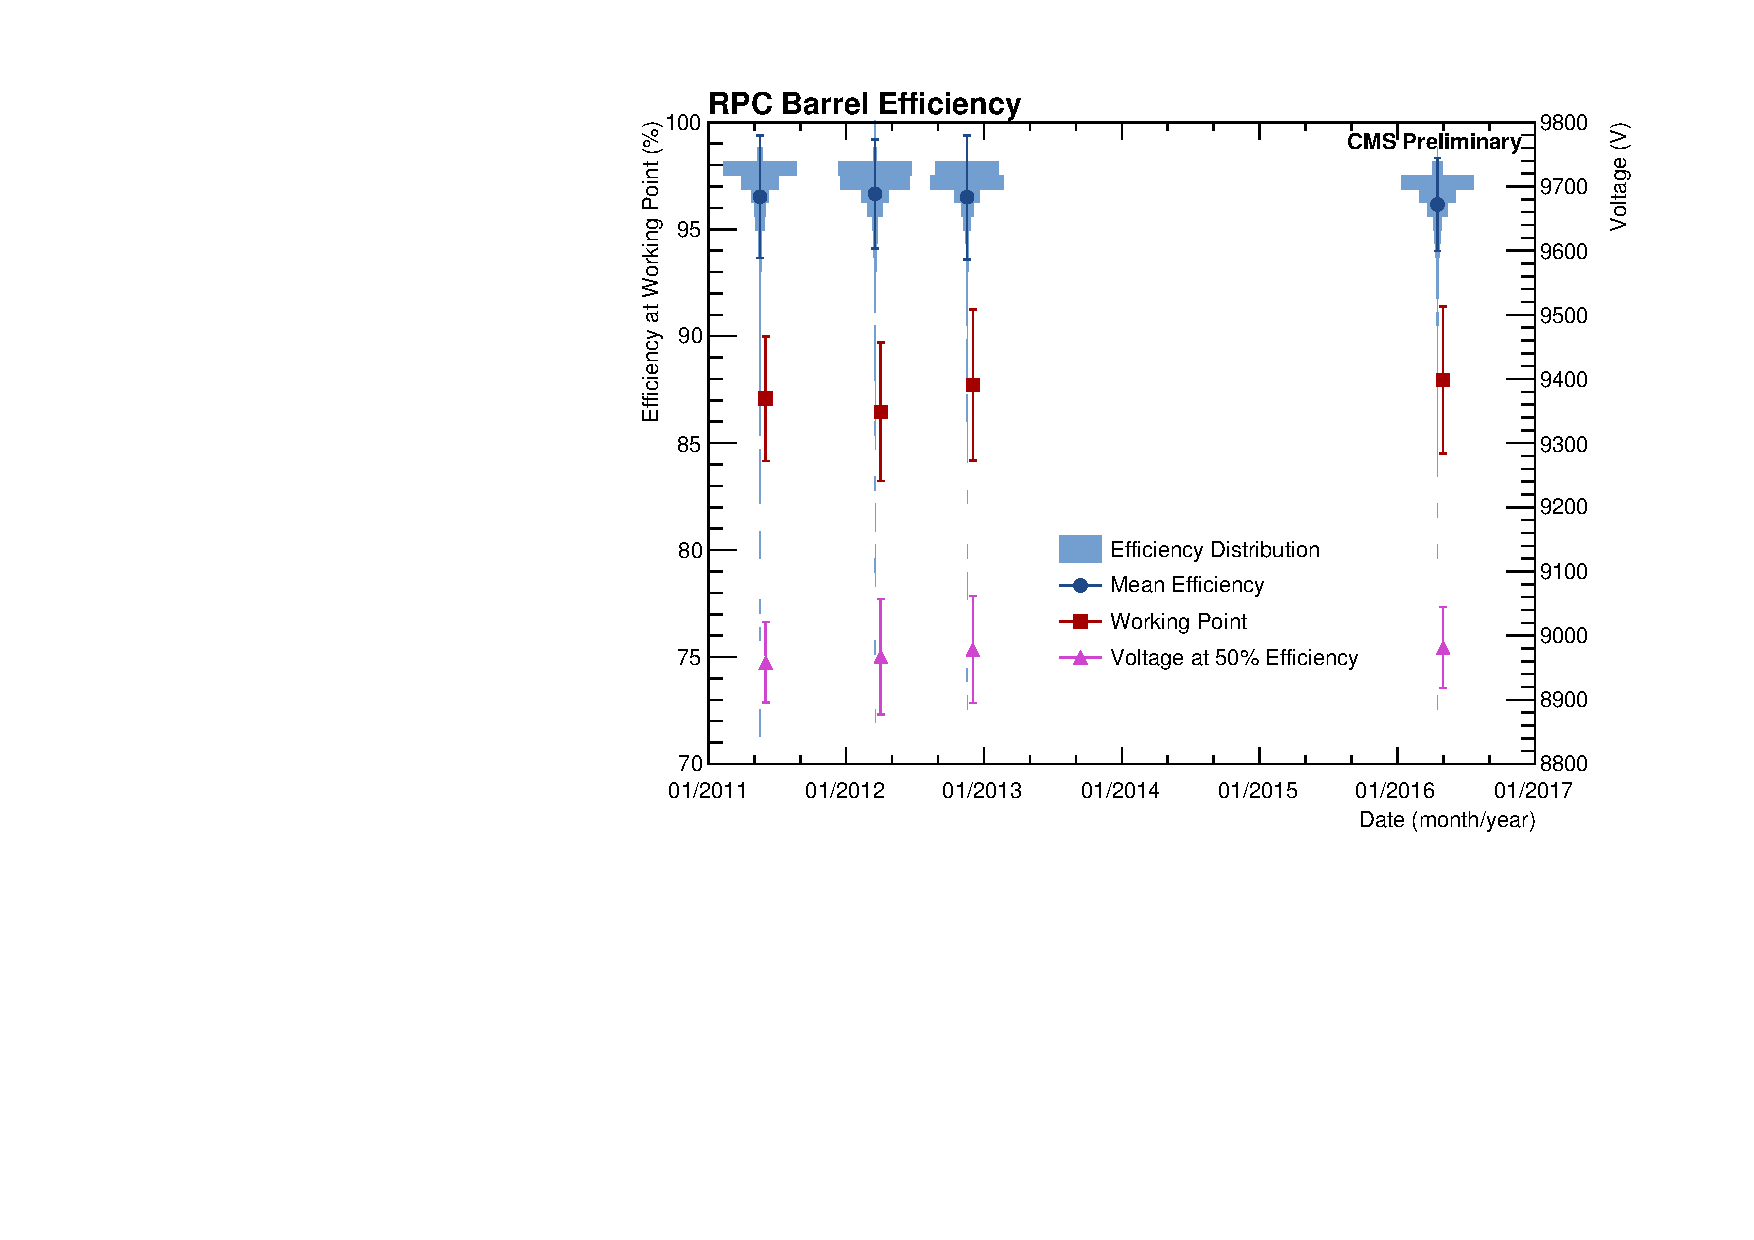
\includegraphics[width = 0.7\plotwidth]{fig/chapt4/HVScanSummaryBarrel.pdf}
			\caption{\label{fig:CMSRPCperf:A}}
		\end{subfigure}
		\begin{subfigure}{0.5\linewidth}
			\centering
			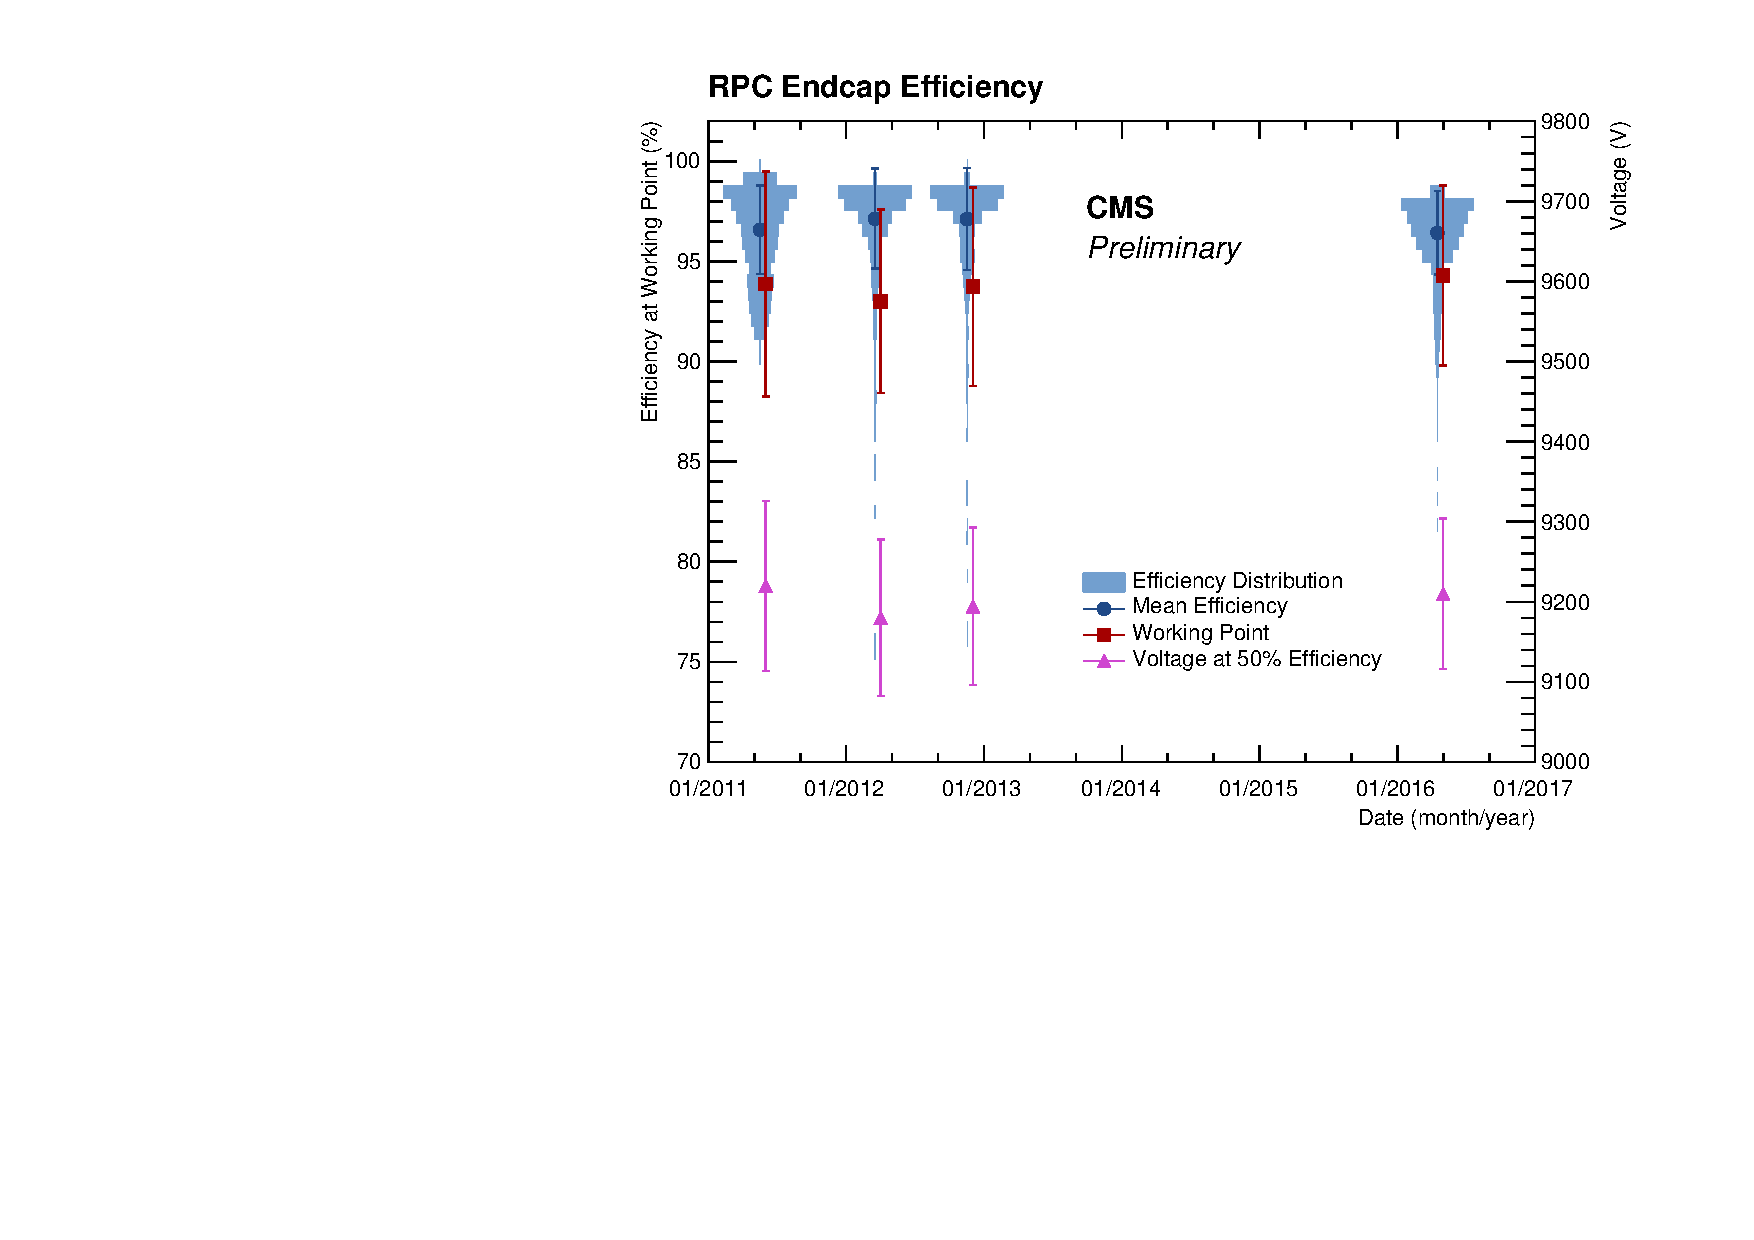
\includegraphics[width = 0.7\plotwidth]{fig/chapt4/HVScanSummaryEndcap.pdf}
			\caption{\label{fig:CMSRPCperf:B}}
		\end{subfigure}
		\caption{\label{fig:CMSRPCperf} Evolution of the efficiency, working voltage, and voltage at 50\% of maximum efficiency for CMS Barrel (Figure~\ref{fig:CMSRPCperf:A}) and Endcap (Figure~\ref{fig:CMSRPCperf:B}) RPCs obtained through yearly voltage scans since 2011. The working voltage of each RPC is updated after each voltage scan to ensure optimal operation~\cite{SHAH2018}.}
	\end{figure}
	
	It was already discussed that in the future, it is likely that the use of freon gases could be banned. As potential replacement for tetrafluoroethane was proposed the trifluoroiodomethane ($CF_3I$), a molecule with similar properties than $CF_3Br$ which was replaced by the tetrafluoroethane, and the 1,3,3,3-tetrafluoropropene ($C_3H_2F_4$ or HFO-1234re), a molecule with similar properties than the actual tetrafluoroethane and proposed as a replacement in refrigirating and air conditioning systems~\cite{HFO2015}. These 2 gases have stronger quenching properties than $C_2H_2F_4$ which means a much stronger electric field needs to be applied on the parallel electrodes of the RPCs in order to reach full efficiency. But the power supply system of CMS RPC is limited to \SI{15}{kV} and so is ATLAS power supply system which is participating in a joined R\&D. As can be seen from Figure~\ref{fig:RPC-eco}, reducing the working voltage was achieved by mixing the potential replacements together with $CO_2$. Introducing carbon dioxide into the mixture while keeping similar levels of isobutane and $SF_6$ increases the streamer probability and the best candidate identified for a compromise in between low enough working voltage and acceptable levels of streamers corresponds to a mixture containing 50\% of $CO_2$, 45\% of HFO, 4\% of isobutane and 1\% of $SF_6$ but is not yet considered satisfactory. On the other hand, no good replacement for $SF_6$ has yet been identified. With its very high \acl{GWP} (23900), even small fraction of this gas in the mixture (it only represents 0.3\% of CMS standard mixture but more than 5\% of its overall GWP) substantially increase the danger for the environment. Although finding a replacement for this gas is less critical than for the tetrafluoroethane composing more than 90\% of usual RPC standard mixtures, the problem will need to be addressed.
	
	\subsection{Detector designs and performance}
	\label{chapt4:ssec:design}
	
	Different RPC design have been used and each of them present its own advantages. Historically, the first type of RPC to have been developed is what is now referred to as \textit{narrow gap} RPC~\cite{SANTONICO81,ZEBALLOS96COMP}.
	
	\begin{figure}[H]
		\centering
		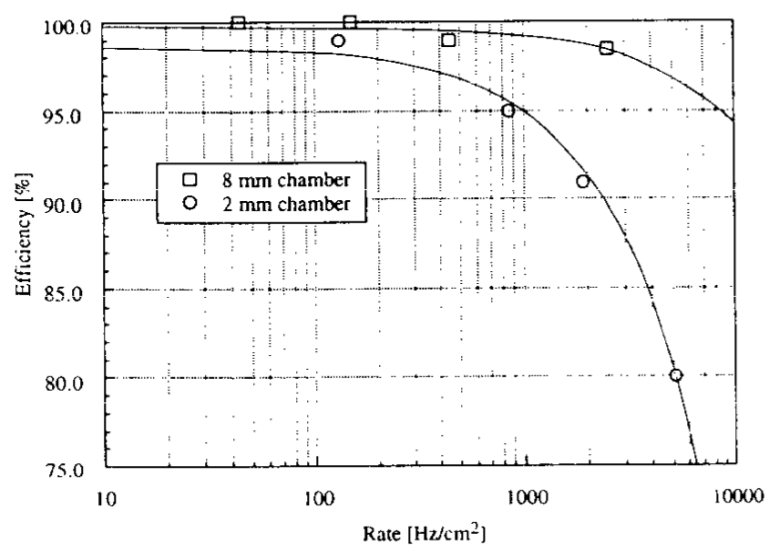
\includegraphics[width = 0.7\plotwidth]{fig/chapt4/Gap-width-rate-cap.png}
		\caption{\label{fig:GapWidthRate} Comparison of the rate capability of \SI{8}{mm} and \SI{2}{mm} wide RPCs. The lines are linear fits on the data~\cite{ZEBALLOS96COMP}.}
	\end{figure}
	
	\begin{figure}[H]
		\hspace*{-0.05\plotwidth}
		\begin{subfigure}{0.5\linewidth}
			\centering
			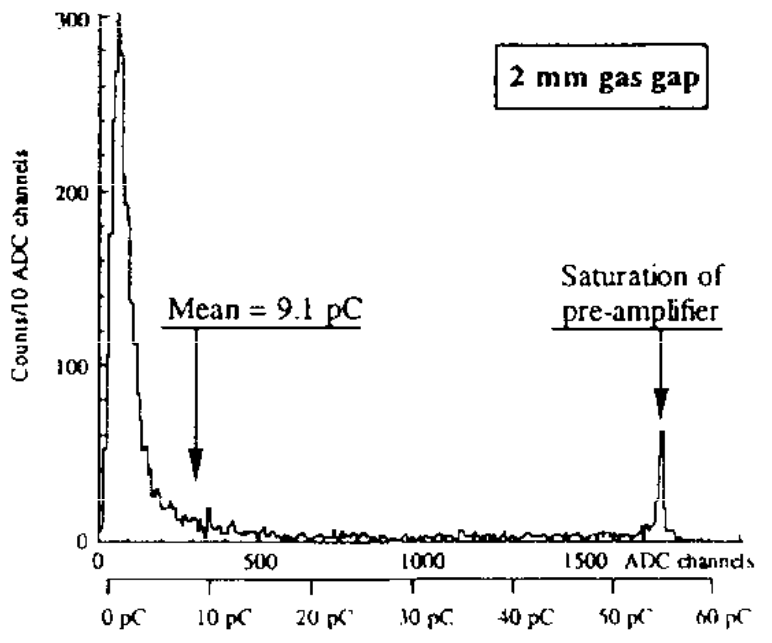
\includegraphics[width = 0.5\plotwidth]{fig/chapt4/Fast-charge-2mm.png}
			\caption{\label{fig:GapWidthCharge:A}}
		\end{subfigure}
		\begin{subfigure}{0.5\linewidth}
			\centering
			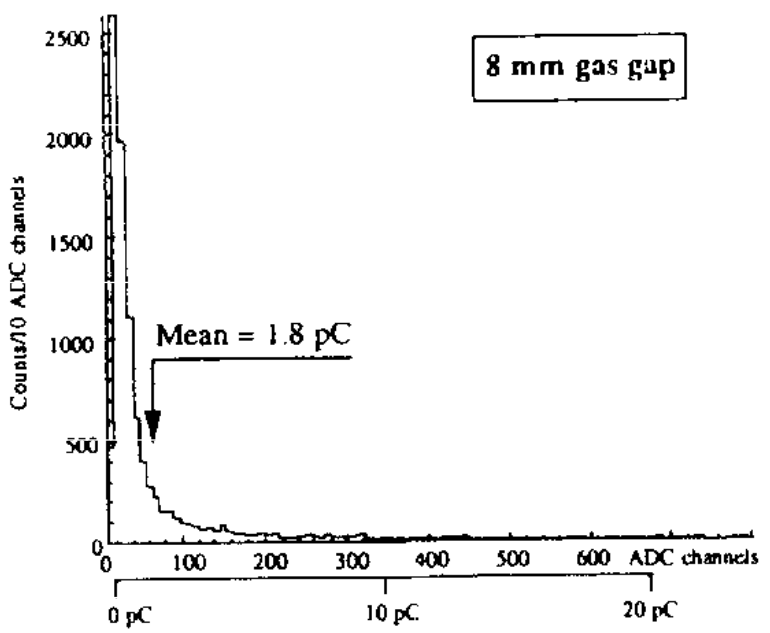
\includegraphics[width = 0.5\plotwidth]{fig/chapt4/Fast-charge-8mm.png}
			\caption{\label{fig:GapWidthCharge:B}}
		\end{subfigure}
		\begin{subfigure}{\linewidth}
			\centering
			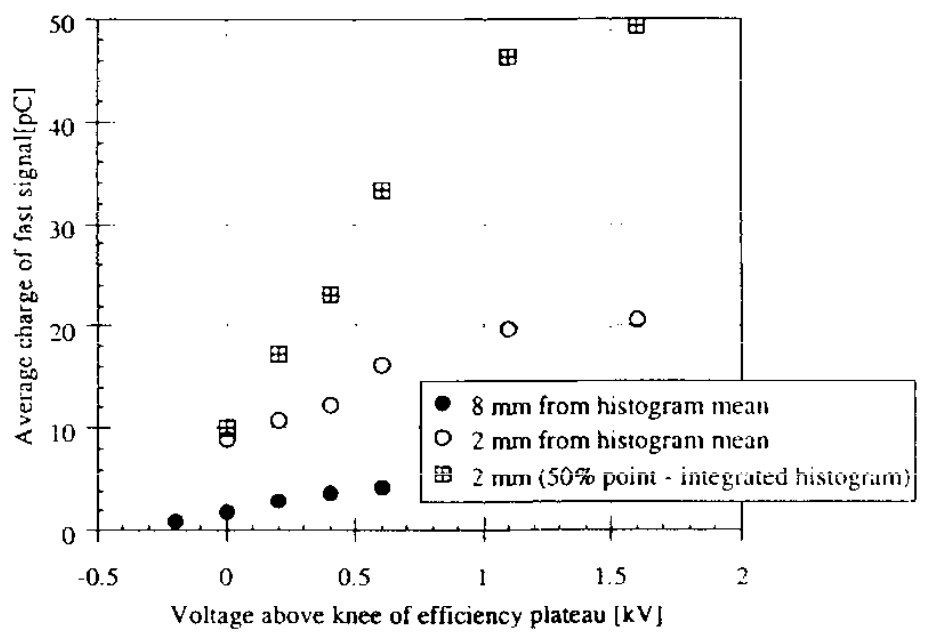
\includegraphics[width = 0.7\plotwidth]{fig/chapt4/Fast-charge-evolution.png}
			\caption{\label{fig:GapWidthCharge:C}}
		\end{subfigure}
		\caption{\label{fig:GapWidthCharge} Distributions of the induced charge of fast signals on \SI{2}{mm} (Figure~\ref{fig:GapWidthCharge:A}) and \SI{8}{mm} (Figure~\ref{fig:GapWidthCharge:B}) RPCs exposed to a radiation rate of \SI{100}{Hz/cm^2}. Average induced charge of fast signals as a function of the high voltage applied on \SI{2}{mm} and \SI{8}{mm} RPCs (Figure~\ref{fig:GapWidthCharge:C}). In the case of the \SI{2}{mm} RPC, a saturation of the pre-amplifier was observed. The average of the distribution is underestimated and the median is showed together with the average to account for this bias~\cite{ZEBALLOS96COMP}.}
	\end{figure}
	
	After the avalanche mode has been discovered~\cite{CROTTY93}, it has been showed that increasing the width of the gas gap lead to higher rate capability, due to lower charge deposition per avalanche, and lower power dissipation~\cite{ZEBALLOS96COMP}, as is showed in Figures~\ref{fig:GapWidthRate} and \ref{fig:GapWidthCharge}. The distance in between the electrode being greater, a weaker electric field can be applied and a lower gain used as a longer gas volume will contribute to the signal induction on the read-out circuit. Nevertheless, by increasing the gas gap width, the time resolution of the detector decreases. This is a natural result if the increase of active gas volume in the detector is taken into account. Indeed, for a given detection threshold on the induced charge per signal, only the small fraction of gas closest to the cathode will provide enough gain to have a detectable signal. In the case of a wider gas volume, the active region is then larger and a larger time jitter is introduced with the variation of starting position of the avalanche, as discussed in~\cite{ZEBALLOS96MRPC} and showed in Figure~\ref{fig:GapWidthTime}.
	
	\begin{figure}[H]
		\centering
		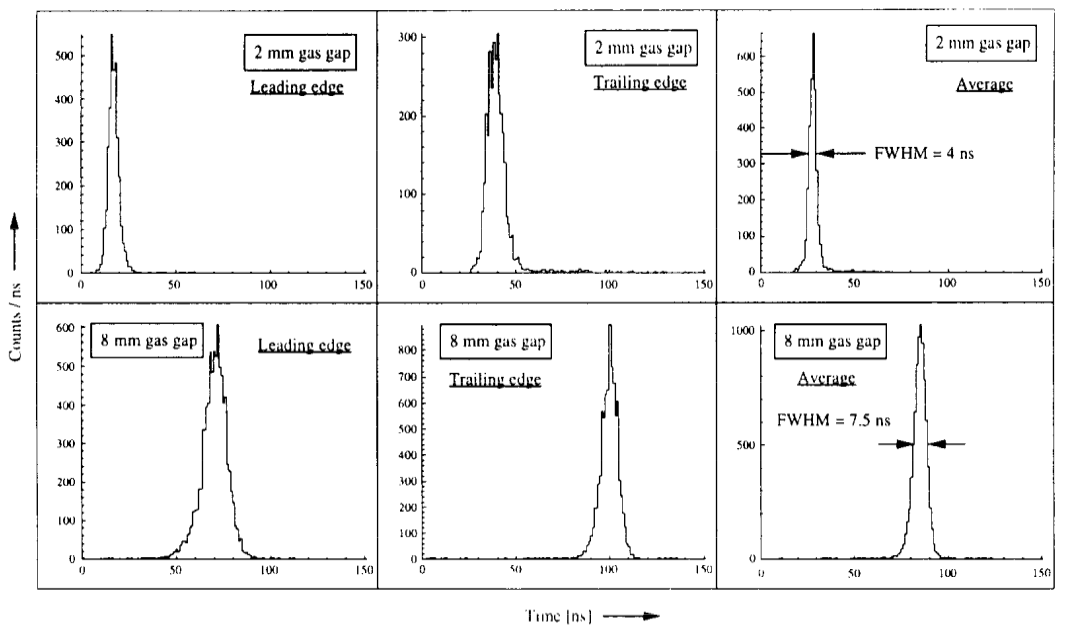
\includegraphics[width = \linewidth]{fig/chapt4/Time-res-gap-width.png}
		\caption{\label{fig:GapWidthTime} Time distributions of the leading, trailing, and average of both leading and traling edges for \SI{2}{mm} (top row) and \SI{8}{mm} (bottom row) RPCs exposed to a \SI{100}{Hz/cm^2} radiation rate. The data was collected with RPCs operated at the voltage corresponding to the knee of the efficiency distribution, defined as the point where 95\% of the maximum efficiency is obtained~\cite{ZEBALLOS96COMP}.}
	\end{figure}
	
	To improve both the time resolution and the rate capability, different methods were used trying to take advantage of both narrow and wide gap RPCs into a single design. Thus, double gap RPCs, combining two narrow gaps into a single detector to increase the effective sensitive volume, and multigap RPCs, which divided the large volume of a wide gap RPC into thinner sub-gaps by adding intermediate electrodes in between the cathode and anode to improve the time resolution by mimicking narrow gap RPCs, were developed starting from the middle of the 90s.
	
		\subsubsection{Double gap RPC}
		\label{chapt4:sssec:DGRPC}
	
	Made out of 2 narrow RPC detectors stacked on top of each other as shown in Figure~\ref{fig:DGLayout}, this detector layout, popularized by the two multipurpose experiments CMS~\cite{MUONTDR} and ATLAS~\cite{ATLASTDR} at LHC, can be used as an OR system in which each individual chamber participates in the ouput signal and increases the overall sensitive volume of the detector apparatus. Keeping the copper strip read-out system at the ground, CMS and ATLAS, due to different goals, have chosen different designs as CMS RPCs possess a 1D read-out while ATLAS RPCs offer a 2D read-out. The difference comes from placing the read-out in between the gaps, the anodes facing each other, or to have both RPC gaps in between 2 layers of read-out panels, one along the X-axis and one along the Y-axis, the cathodes facing each other.
	
	\begin{figure}[H]
		\centering
		\includegraphics[width = \plotwidth]{fig/chapt4/Double_gap_layouts.pdf}
		\caption{\label{fig:DGLayout} Possible double-gap RPC layouts: a) "standard" 1D double-gap RPC, as used in CMS experiment, where the anodes are facing each other and a 1D read-out plane is sandwished in between them,  b) double read-out double-gap RPC as used in ATLAS experiment, where the cathodes are facing each other and 2 read-out planes are used on the outter surfaces. This last layout can offer the possibility to use a 2D reconstruction by using orthogonal read-out planes.}
	\end{figure}
	
	\begin{figure}[H]
		\begin{subfigure}{0.33\linewidth}
			\centering
			\hspace*{-0.3\linewidth}
			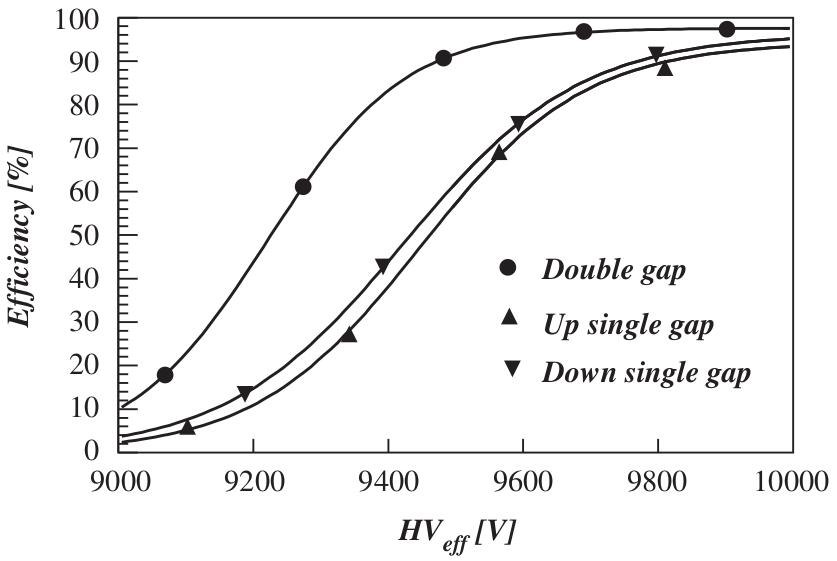
\includegraphics[height = 3.6cm]{fig/chapt4/Double-gap-Sigmoid.png}
			\caption{\label{fig:DoubleGap:A}}
		\end{subfigure}
		\begin{subfigure}{0.33\linewidth}
			\centering
			\hspace*{-0.1\linewidth}
			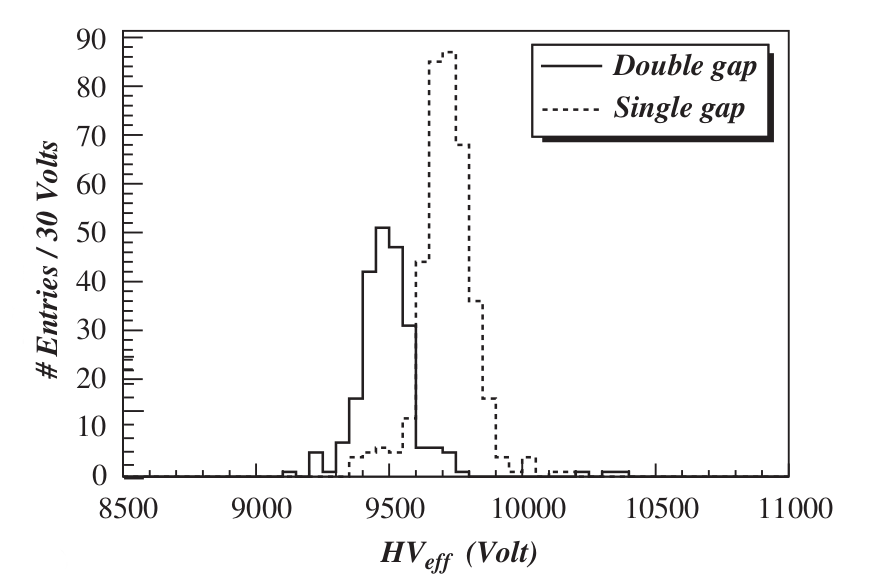
\includegraphics[height = 3.6cm]{fig/chapt4/Double-gap-Eff-95.png}
			\caption{\label{fig:DoubleGap:B}}
		\end{subfigure}
		\begin{subfigure}{0.33\linewidth}
			\centering
			\hspace*{0.03\linewidth}
			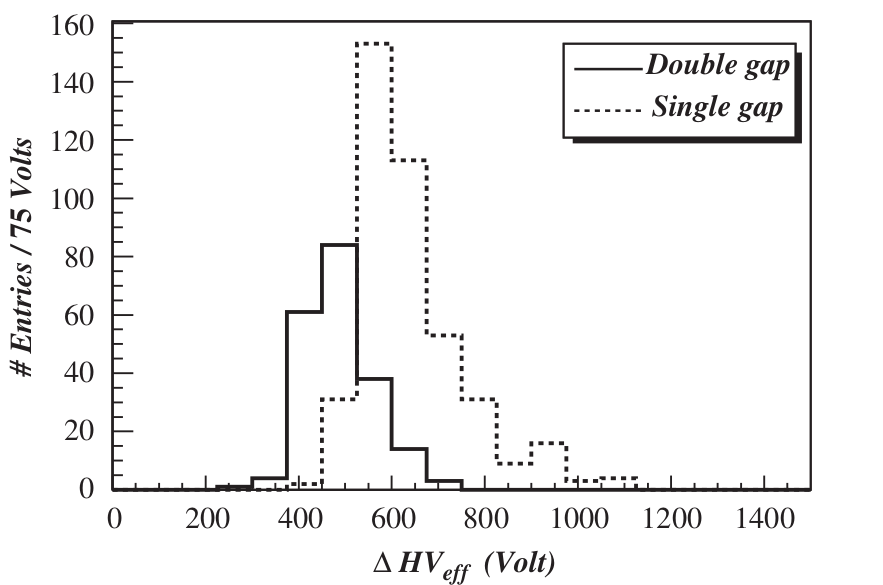
\includegraphics[height = 3.6cm]{fig/chapt4/Double-gap-Eff-Delta-90-10.png}
			\caption{\label{fig:DoubleGap:C}}
		\end{subfigure}
		\caption{\label{fig:DoubleGap} Comparison of performance of CMS double and single gap RPCs using cosmic muons~\cite{ABBRESCIA2005}. Figure~\ref{fig:DoubleGap:A}: Comparison of efficiency sigmoids. Figure~\ref{fig:DoubleGap:B}: Voltage distribution at 95\% of maximum efficiency. Figure~\ref{fig:DoubleGap:C}: $\Delta^{90\%}_{10\%}$ distribution.}
	\end{figure}
	
	The gain of such a detector is reduced by a factor 2 with respect to single-gap RPCs with an efficiency plateau reached at lower voltage, as visible on Figure~\ref{fig:DoubleGap}, due to the two gas gaps contributing to the signal formation and offering a dynamic range closer to witch of a wide gap RPC. A double gap is then fully efficient while the individual RPC gaps composing it are only 70 to 80\% efficient. Naturally, by operating the double gap at a lower voltage, the rate capability in found to be increased as the induced charge per gap is then lower than in the can than a single gap detector also leading to a reduction of the streamer probability and a better extraction of the fast charge of the total signal as could be seen through previously presented Figure~\ref{fig:FreonArgonFastCharge}.
	
		\subsubsection{Multigap RPC (MRPC)}
		\label{chapt4:sssec:MRPC}
	
	MRPCs are layouts in which floating sub electrode plates are placed into a wide gap RPC to divide the gas volume and create a sum of narrow gaps~\cite{ZEBALLOS96MRPC,WILLIAMS98}. Similarly to the double gap RPC for which the gain could be reduced by increasing the dynamic range, the multigap reduces the gain while keeping a total dynamic range similar to which of a wide gap RPC by reducing the size of each individual sub-gap composing the detector. The dynamic range, associated to the sensitive volume, and the comparison of each detector layout to the wide gap RPC is showed in Figure~\ref{fig:RPClayouts}.
	
	\begin{figure}[H]
		\centering
		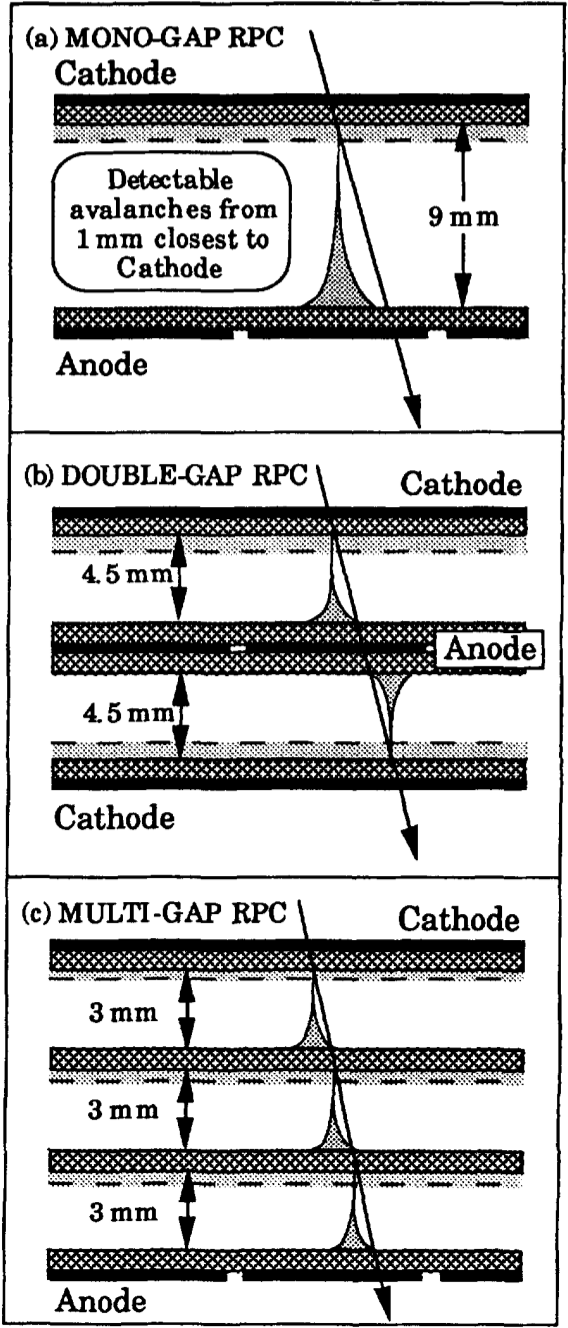
\includegraphics[width = 0.5\plotwidth]{fig/chapt4/RPC-layouts-dyn-range.png}\\
		\caption{\label{fig:RPClayouts} Representation of different RPC layouts (wide gap on Figure (a), double gap on Figure (b) and multigap on Figure (c)), of the corresponding sensitive volume in gray, and of the associated avalanche size~\cite{WILLIAMS98}.}
	\end{figure}
	
	By operating the detector with thinner gaps, the time resolution is improved. Comparatively to the time resolution presented in Figure~\ref{fig:GapWidthTime} for the wide gap RPC of \SI{8}{mm}, a complementary study was conducted on multigaps using two \SI{4}{mm} and four \SI{2}{mm} subgaps and showed, via Figure~\ref{fig:MRPCTimeRes}, an improvement of the time resolution with the reduction of the gap width and of the number of gaps while the same sensitive volume was kept~\cite{WILLIAMS98}.
	
	\begin{figure}[H]
		\begin{subfigure}{\linewidth}
			\centering
			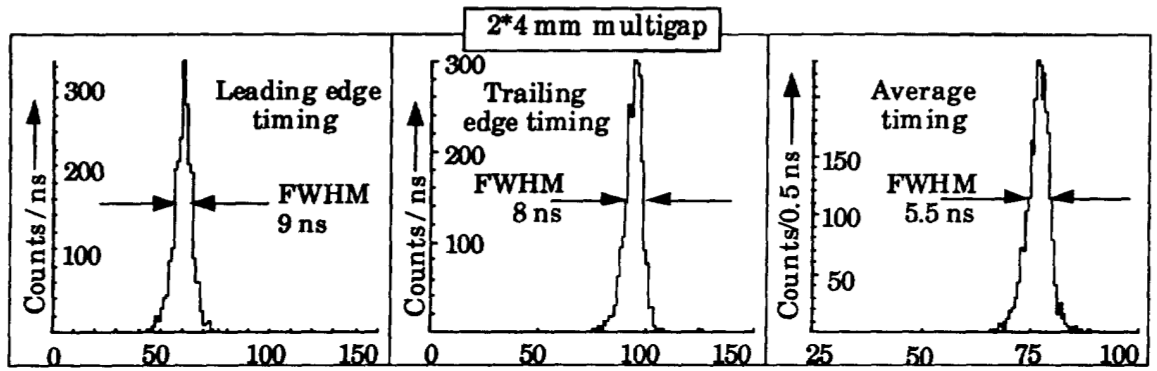
\includegraphics[width = \plotwidth]{fig/chapt4/MRPC-2-4mm-time-res.png}
			\caption{\label{fig:MRPCTimeRes:A}}
		\end{subfigure}
		\begin{subfigure}{\linewidth}
			\centering
			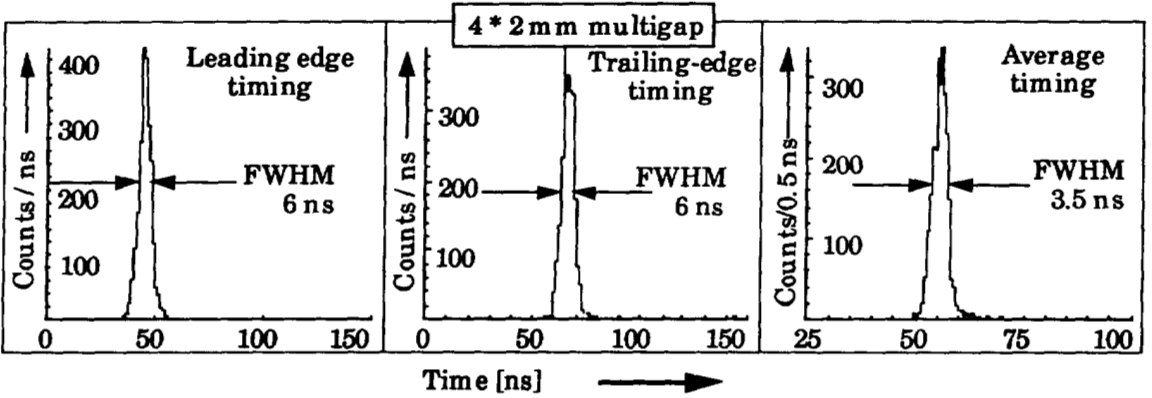
\includegraphics[width = \plotwidth]{fig/chapt4/MRPC-4-2mm-time-res.png}
			\caption{\label{fig:MRPCTimeRes:B}}
		\end{subfigure}
		\caption{\label{fig:MRPCTimeRes} Time distributions of the leading, trailing, and average of both leading and traling edges for multigap RPCs consisting in two \SI{4}{mm} (Figure~\ref{fig:MRPCTimeRes:A}) and four \SI{2}{mm} (Figure~\ref{fig:MRPCTimeRes:B}) exposed to a \SI{100}{Hz/cm^2} radiation rate. The data was collected with RPCs operated at the voltage corresponding to the knee of the efficiency distribution, defined as the point where 95\% of the maximum efficiency is obtained~\cite{WILLIAMS98}.}
	\end{figure}
	
	\begin{figure}[H]
		\begin{subfigure}{0.4\linewidth}
			\centering
			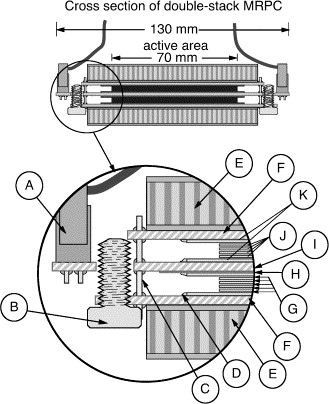
\includegraphics[width = 0.45\plotwidth]{fig/chapt4/MRPC-Layout.png}
			\caption{\label{fig:ALICEMRPC:A}}
		\end{subfigure}
		\begin{subfigure}{0.6\linewidth}
			\centering
			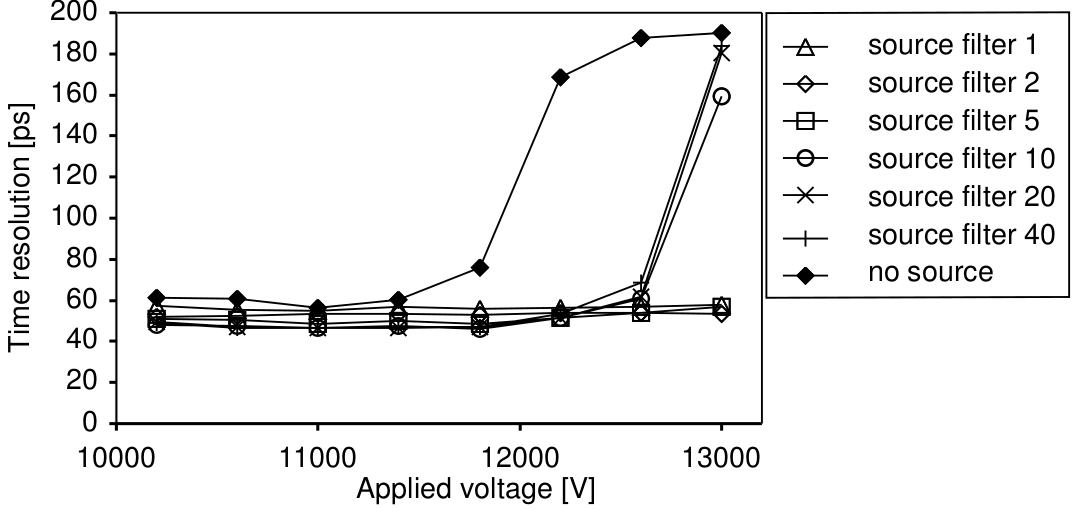
\includegraphics[width = 0.7\plotwidth]{fig/chapt4/ALICE-2002-time-res.png}
			\caption{\label{fig:ALICEMRPC:B}}
		\end{subfigure}
		\caption{\label{fig:ALICEMRPC} Presentation of a study of a possible ALICE MRPC cell using \SI{250}{\micro m} gas gaps, \SI{620}{\micro m} outer glass electrodes, and \SI{550}{\micro m} inner floating electrodes (Figure~\ref{fig:ALICEMRPC:A}), and of its time resolution performance as a function of the applied high voltage for different radiation levels referred through different filter settings of the \SI{740}{GBq} $^{137}Cs$ source the former CERN GIF facility~\cite{ALICE2002}.}
	\end{figure}
	
	After the problem of streamers was solved by adding $SF_6$ into the gas mixture, the size of the MRPCs decreased as the research groups started applying the concept of dividing the gas volume into subvolumes to the narrow gap RPCs leading to the now widely used micro gap MRPCs. The time resolution of such a detector can reach of few tens of \si{ps}, with gas gaps of the order of a few hundred \si{\micro m} as showed in Figure~\ref{fig:ALICEMRPC} representing a single cell of ALICE \acf{ToF} system consisting of double MRPCs, as it was studied in the early 2000s~\cite{ALICE2002}.
	
	Sometimes used as a double multigap RPC, taking advantage of the OR of double gap RPCs to both be able to operate a higher number of gaps while keeping a reasonable high voltage applied in between the cathode and anode and to further reduce the gain, the MRPC is mainly used as ToF detector~\cite{ALICE2002,START2002,BESIII2014,CBM2007,MPD2016} due to its excellent timing properties that allow to perform particle identification as explained by Williams in~\cite{WILLIAMS2012}. The principle of particle identification using ToF is simply the measurement of the velocity of a particle. Indeed, particles are defined by their mass (for the parameter of interest here, their electric charge being measured using the bending angle of the particles traveling through a magnetic field) and this mass can be calculated by measuring the velocity $\beta$ and momentum of the particle:
	
	\begin{equation}
		\beta = \frac{p}{\sqrt{p^2 + m^2}}
	\end{equation}
	
	Intuitively, it is trivial to understand that 2 different particles having the same momentum will have a different velocity due to the mass difference and thus a different flight time $T_1$ and $T_2$ through the detector and this is used to separate and identify particles. The better the time resolution of the ToF system used, the stronger will the separation be:
	
	\begin{equation}
		T = \frac{L}{v} = \frac{L}{c\cdot\beta}, \quad \Delta T = T_1 - T_2 = \frac{L}{c}\left(\sqrt{1+m_1^2/p^2} - \sqrt{1+m_2^2/p^2}\right) \cong (m_1^2 - m_2^2)\frac{L}{2cp^2}
	\end{equation}
	
	An example of particle identification is given for the case of STAR experiment in Figure~\ref{fig:ParticleID}.
	
	\begin{figure}[H]
		\centering
		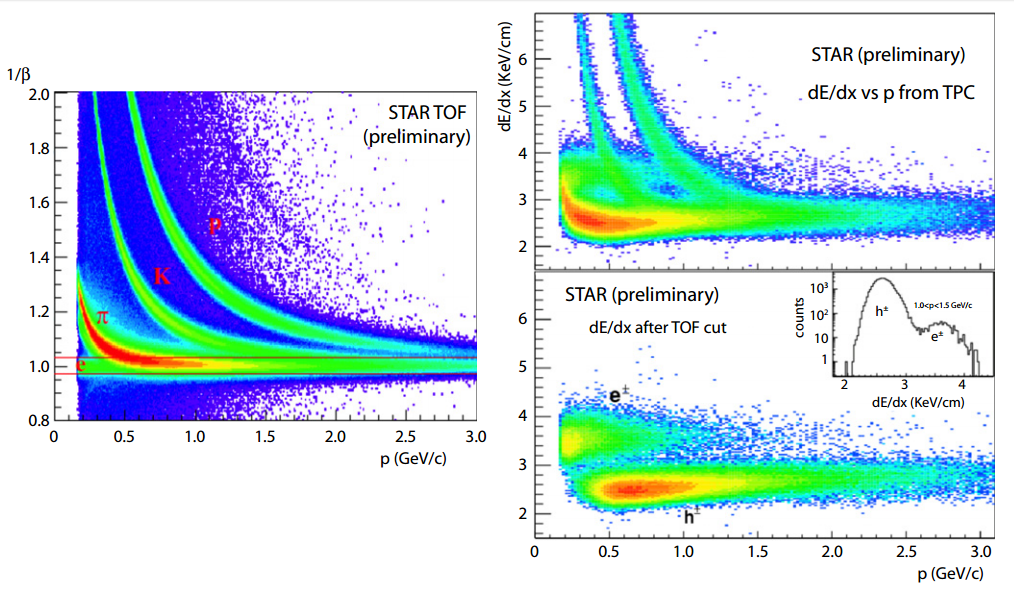
\includegraphics[width = \plotwidth]{fig/chapt4/STAR-ToF.png}\\
		\caption{\label{fig:ParticleID} Particle identification applied to electrons in the STAR experiment. The identification is performed combining ToF and $dE/dx$ measurements~\cite{WILLIAMS2012}.}
	\end{figure}
	
	Taking into account the distortion effect on the electric field inside of a MRPC built using micro gaps due to the exposition to irradiation, distortion that can be understood by monitoring the current drawn by the detector which should stay constant at constant electric field, another benefice of using such small gas gaps is the strong reduction of the average avalanche volume and thus of the blind spot on MRPCs leading to an improved rate capability. Multigaps can sustain backgrounds of several \si{kHz/cm^2} as demonstrated in Figure~\ref{fig:MRPCRate}.
	
	\begin{figure}[H]
		\centering
		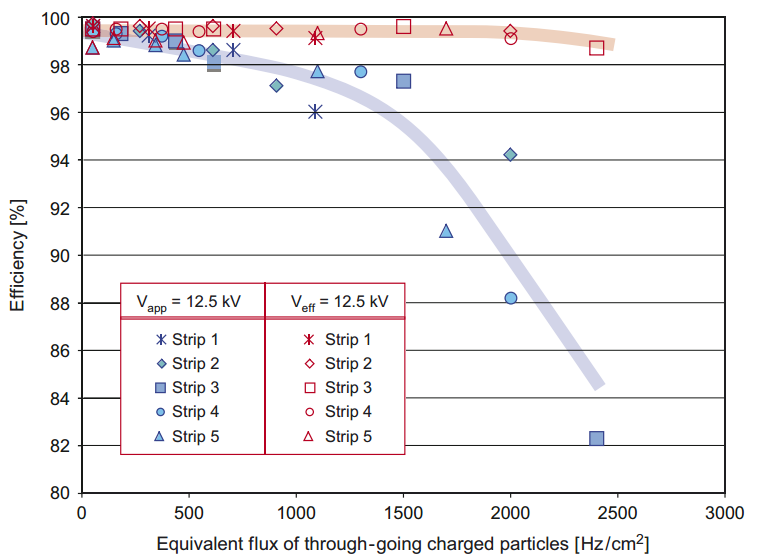
\includegraphics[width = 0.7\plotwidth]{fig/chapt4/ALICE-Rate_Capability.png}\\
		\caption{\label{fig:MRPCRate} Comparison of the detector performance of ALICE ToF MRPC~\cite{ALICI2007} at fixed applied voltage (in blue) and at fixed effective voltage (in red). The effective voltage is kept fixed by increasing the applied voltage accordingly to the current drawn by the detector.}
	\end{figure}
	
		\subsubsection{Charge distribution and performance limitations}
		\label{chapt4:sssec:charge}
		
	{\color{blue}\textbf{[This part could be moved in the next section of the chapter and deepened using the perspective of the avalanche physics.]}}
		
	The direct consequence of the different RPC layouts is a variation of intrinsic time resolution of the RPC as the gap size decreases and of the rate capability when the deposited charge per event is spread over a larger number of amplification volumes, allowing for a reduction of the overall gain of the detectors which is replaced by an on-electronics pre-amplification of the signals. in this sense, an advantage is given to multigaps whose design use sub-millimeter gas volumes providing very consistent signals.
	
	From the charge spectrum point of view, each layout has its own advantages. When the double-gap has the highest induced over drifting charge ratio, as seen in Figure~\ref{fig:ChargeRatio}, the multigap has a charge spectrum strongly detached from the origin, as visible in Figure~\ref{fig:ChargeSpectra}. A high induced over drifting charge ratio means that the double gap can be safely operated at high threshold or that at similar threshold it can be operated with a twice smaller drifting charge, meaning a higher rate capability if operated with sensitive enough electronics. On the other hand, the strong detachment of the charge spectrum from the origin in the MRPC case allows to reach a higher efficiency with increasing threshold as most of the induced charge is not low due to the convolution of several single gap spectra. The range of stable efficiency increases with the number of gap, as presented in Figure~\ref{fig:EffThreshold}.
	
	\begin{figure}[H]
		\centering
		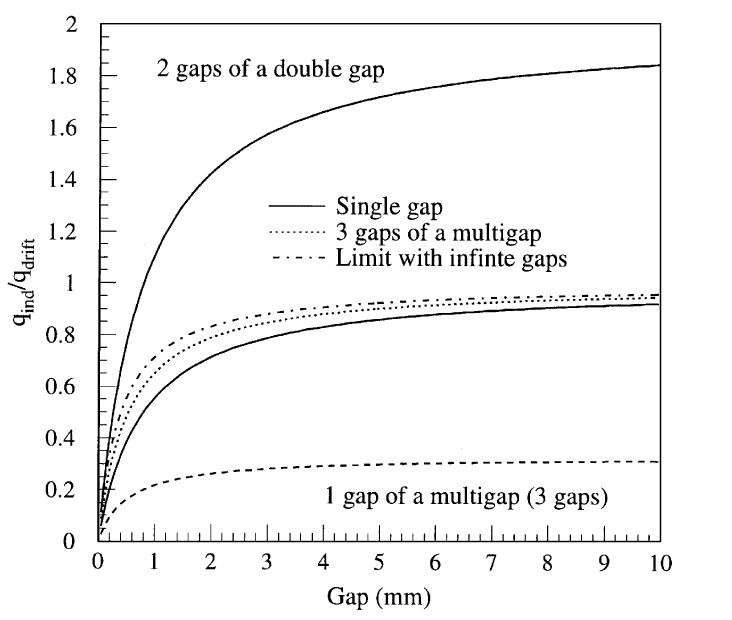
\includegraphics[width = 0.6\plotwidth]{fig/chapt4/Layout_charge_ratio.png}\\
		\caption{\label{fig:ChargeRatio} Ratio between total induced and drifting charge have been simulated for single gap, double-gap and multigap layouts~\cite{ABBRESCIA99}. The total induced charge for a double-gap RPC is a factor 2 higher than for a multigap.}
	\end{figure}
	
	\begin{figure}[H]
		\centering
		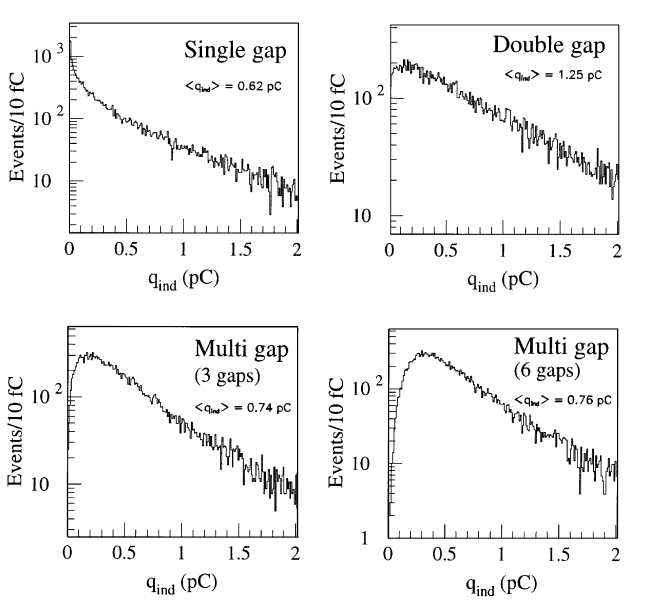
\includegraphics[width = \plotwidth]{fig/chapt4/Layout_charge_distributions.png}\\
		\caption{\label{fig:ChargeSpectra} Charge spectra have been simulated for single gap, double-gap and multigap layouts~\cite{ABBRESCIA99}. It appears that when single gap shows a decreasing spectrum, double and multigap layouts exhibit a spectrum whose peak is detached from the origin. The detachment gets stronger as the number of gaps increases.}
	\end{figure}
	
	\begin{figure}[H]
		\centering
		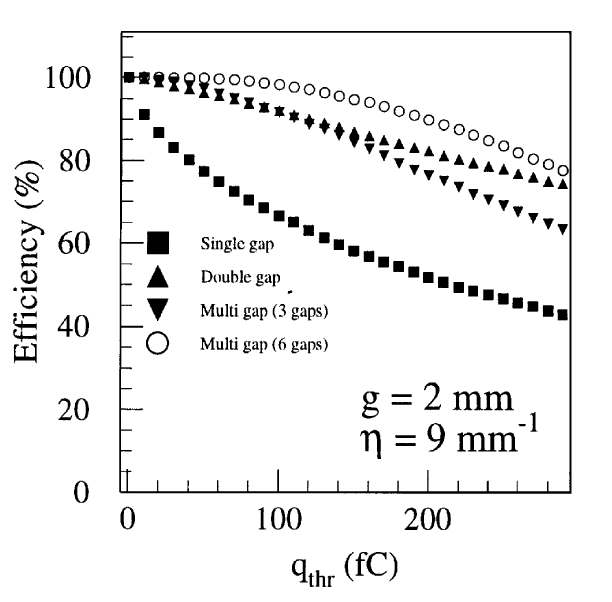
\includegraphics[width = 0.6\plotwidth]{fig/chapt4/Layout_eff_vs_thr.png}\\
		\caption{\label{fig:EffThreshold} The maximal theoretical efficiency is simulated for single gap, double-gap and multigap layouts~\cite{ABBRESCIA99} at a constant gap thickness of \SI{2}{mm} and using an effective Townsend coefficient of \SI{9}{mm^{-1}}.}
	\end{figure}

\section{Signal formation}
\label{chapt4:sec:signal}
	
	\begin{figure}[H]
		\centering
		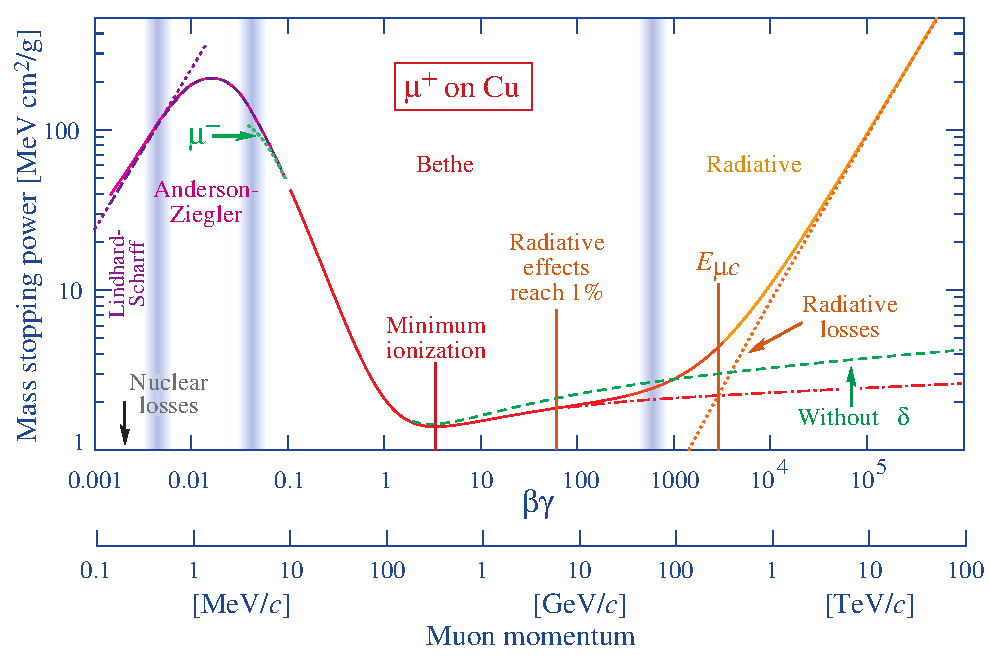
\includegraphics[width = \plotwidth]{fig/chapt4/rpp_icru49_cu_col.pdf}\\
		\caption{\label{fig:enerlylosscopper} Mass stopping power as a function of $\beta\gamma = p/Mc$ for positive muons in copper~\cite{PDG2016}. The total stopping power is indicated with solid line and local components with dashed lines. the vertical bands are used to indicate boundaries between different approximations used at different energy range.}
	\end{figure}

	The physics of Resistive Plate Chambers still is far from being fully understood and work is regularly being accomplished in trying to model these detectors the best way possible by phenomenological models using well-defined physics~\cite{LIPPMANN2003,VINCENT2016,VINCENT2017}. These theoretical works have nevertheless lead to a better understanding of the key principles that account for RPCs signal formation. As previously discussed, the typical mixture of such a detector is in great majority composed by a ionizing gas with some quenching properties and a low ionization potential to easily produce electrons, with the addition of UV quencher and electronegative compounds. The electronic avalanche formation will be triggered by a charged particle passing through the gas, typically a muon in the case of most uses of RPCs. The production of electrons in the gas of a detector is related to the energy lost by the incoming particle traveling through a material medium. The example of the mass stopping power of copper on muons is given in Figure~\ref{fig:enerlylosscopper} on which the different energy loss mechanisms at different energy ranges are visible. Once primary electrons have been freed in the gas volume, the electric field applied in between the electrodes of the RPC will make the charges move and there will be a competition in the gas in between the Townsend and attachment coefficient which describe the evolution of the number of electrons in an avalanche. While drifting through the gas, the electrons are also subjected to diffusion that will affect the evolution of the avalanches. Finally, when the avalanche is big enough, the accumulation of negative (electrons) and positive (ions) charges in the gas volume will start affecting the local electric field. This effect is known as space charge effect.
	
	\subsection{Energy loss at intermediate energies}
	\label{chapt4:ssec:ElossBethe}
	
	Intuitively, a particle traveling through a medium will interact with its components, losing energy. When a muon travels through the gas of a gaseous detector, at the energy range usually observed, it interacts with the molecules of the gas leading to dissipation of the transferred energy in the form of inelastic diffusion or ionization. The photons and electron-ion pairs resulting from these interaction can trigger avalanches in the gas which will contribute to feed the avalanche growth thanks to the strong electric field applied in between the 2 electrodes of a RPC.
	
	The mass stopping power of moderately relativistic ($0.1 \lesssim \beta\gamma \lesssim 1000$) heavy particles ($M \gg m_e$) traveling through a medium via excitation and ionization processes was studied by Bethe in 1930~\cite{BETHE1930} and is well described by the so called the Bethe Formula given in Equation~\ref{eq:bethe}.
	
	\begin{equation}
	\label{eq:bethe}
	\left\langle-\frac{dE}{dx}\right\rangle = Kz^2\frac{Z}{A}\frac{1}{\beta^2}\left(\frac{1}{2}ln\frac{2m_ec^2\beta^2\gamma^2W_{max}}{I^2}-\beta^2-\delta(\beta\gamma)\right)
	\end{equation}
	
	The different parameters used in this equation are
	
	\begin{longtable}{r c l l}
		$E$ &-& incident particle energy $\gamma Mc^2$ & \si{MeV}\\
		$x$ &-& mass per unit area & \si{g.cm^{-2}}\\
		$N_A$ &-& Avogadro's number & 6.022 140 857(74) $\times 10^{23}$\si{mol^{-1}}\\
		$c$ &-& speed of light in vacuum & 299 792 458\si{m.s^{-1}}\\
		$\mu_0$ &-& permeability of free space & 4$\pi\times 10^{-7}$\si{N.A^{-2}}\\
		$\epsilon_0$ &-& permittivity of free space $\epsilon_0 = 1/\mu_0c^2$ & 8.854 187 817 . . . $\times 10^{-12}$\si{F.m^{-1}}\\
		$\alpha$ &-& fine structure constant $\alpha = e^2/4\pi\epsilon_0\hbar c$ & 1/137.035 999 139(31)\\
		$r_e$ &-& classical electron radius $r_e = e^2/4\pi\epsilon_0m_ec^2$ & 2.817 940 3227(19)\si{fm}\\
		$e$ &-& elementary charge of the electron & -1.6021766208(98) $\times 10^{-19}$\si{C}\\
		$m_ec^2$ &-& electron mass $\times c^2$ & 0.510 998 9461(31)\si{MeV}\\
		$K$ &-& constant defined as $K = 4\pi N_A r_e^2 m_ec^2$ & \SI{0.307075}{MeV.mol^{-1}.cm^2}\\
		$z$ &-& charge number of incident particle &\\
		$Z$ &-& atomic number of absorbing medium &\\
		$A$ &-& atomic mass of absorbing medium & \si{g.mol^{-1}}\\
		$\beta$ &-& velocity of particle $\beta = v/c$ &\\
		$\gamma$ &-& Lorentz factor $\gamma = (1-\beta^2)^{-1/2}$&\\
		$W_{max}$ &-& maximum energy transfer through a single collision & \si{MeV}\\
		$I$ &-& mean excitation energy of absorbing medium & \si{eV}\\
		$\delta(\beta\gamma)$ &-& density effect correction to ionization energy loss & \\
	\end{longtable}
	
	\begin{figure}[H]
		\centering
		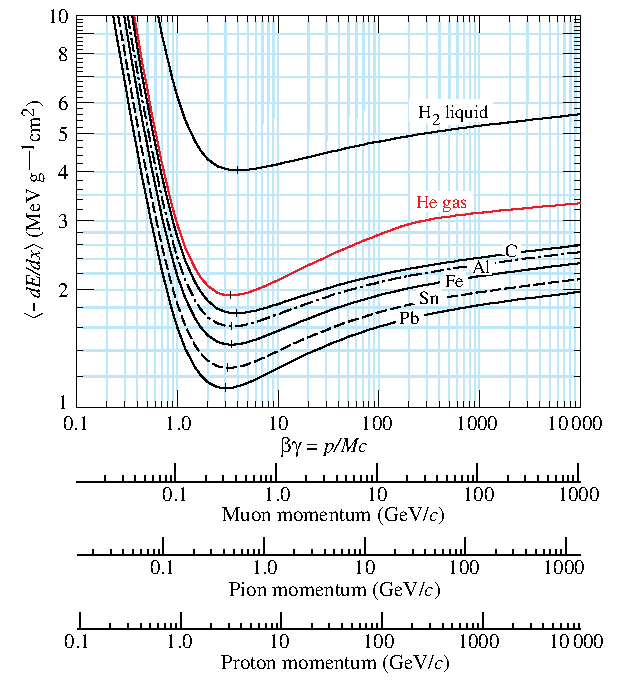
\includegraphics[width = 0.8\plotwidth]{fig/chapt4/dedx_table_98.pdf}\\
		\caption{\label{fig:enerlyloss} Mean mass stopping power for liquid hydrogen, as used in bubble chambers, gaseous helium, carbon, aluminum, iron, tin, and lead without the inclusion of radiative effect at higher $\beta\gamma$ necessary for pions and muons in denser materials~\cite{PDG2016}.}
	\end{figure}
	
	In this equation, the maximum energy transfer $W_{max}$ is defined as function of the incident particle mass $M$, expressed in \si{MeV/c^2}
	
	\begin{equation}
	\label{eq:maxenergytrans}
	W_{max} = \frac{2m_ec^2\beta^2\gamma^2}{1 + 2\gamma m_e/M + (m_e/M)^2}
	\end{equation}
	
	and the mean excitation energy $I$ depends on the absorber and its determination is non-trivial but recommendation are given by the \acf{ICRU} based on experimental measurements and interpolations as showed in Figure~\ref{fig:excitationenergy}.
	
	For the case of copper, the mean stopping power is visible in Figure~\ref{fig:enerlylosscopper}. The mean stopping power corresponding only to the Bethe range for other materials is given in Figure~\ref{fig:enerlyloss} and shows that $\langle-dE/dx\rangle$ is similar for each material with a slow decrease with $Z$. The factor affecting the equation the most is $\beta$ as the dependence on $M$ is introduced at higher energies in the logarithm via the max transfer energy per single collision but in most practicle cases, only the dependence on $\beta$ is considered as most of the relativistic particles are closed to the lowest mean energy loss rate and are referred to as \acf{mip's}. The almost logarithmic relation in between the mean energy loss rate for \acl{mip's} and $Z$ is showed in Figure~\ref{fig:miplossrate}.
	
	\begin{figure}[H]
		\centering
		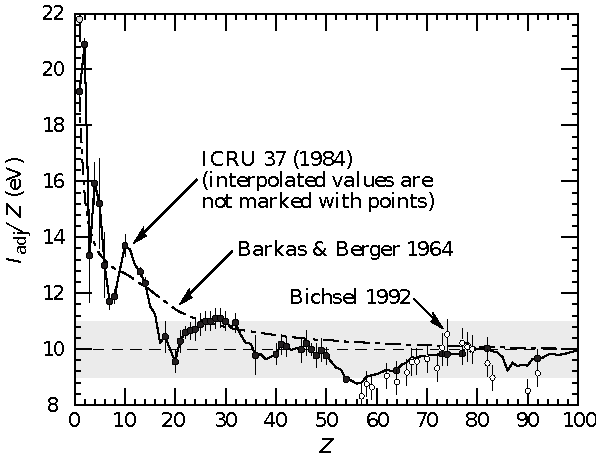
\includegraphics[width = 0.8\plotwidth]{fig/chapt4/Iadj_pegs_adndt.pdf}\\
		\caption{\label{fig:excitationenergy} Mean excitation energies normalized to the atomic number as adopted by the ICRU~\cite{ICRU37,ICRU49,PDG2016}.}
	\end{figure}
	
	\begin{figure}[H]
		\centering
		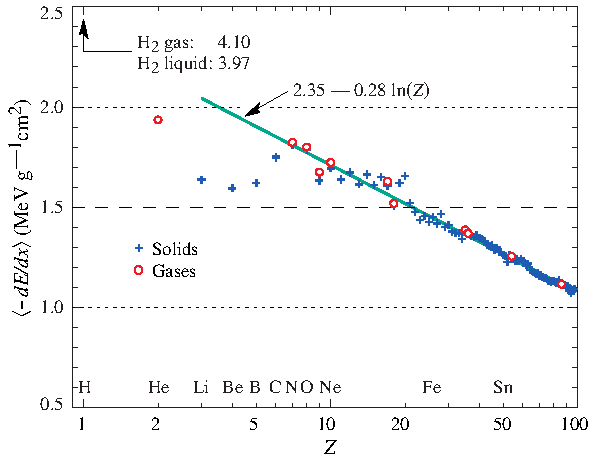
\includegraphics[width = 0.8\plotwidth]{fig/chapt4/dedx_min_06.pdf}\\
		\caption{\label{fig:miplossrate} Mean mass stopping power at minimum ionization as a function of the atomic number~\cite{PDG2016}.}
	\end{figure}
	
	Finally, the term $\delta(\beta\gamma)/2$ corresponds to the density effect correction introduced to account for the polarization of a real media that limits the spatial extension of the electric field of relativistic particles. Indeed, as the energy of a particle increases, the associated electric field will flatten and extend. Due to this effect, the distant collision contribution to Equation~\ref{eq:bethe} will increase as $ln(\beta\gamma)$ but the polarization of the media trunc this rise. At high energies, the correction is given by Equation~\ref{eq:densityeffect}
	
	\begin{equation}
	\label{eq:densityeffect}
	\delta/2 \longrightarrow ln(\hbar\omega_p/I) + ln(\beta\gamma) - 1/2
	\end{equation}
	
	where $\hbar\omega_p$ represents the plasma energy that depends on the electron density of the media and the electron mass and can be calculated as $\sqrt{\rho\langle Z/A \rangle} \times 28.816$ \si{eV}. The introduction of this correction term reduces the increase of the mean stopping power at higher energies as can be seen in Figure~\ref{fig:enerlylosscopper}. Moreover, due to poorer electron density, the effect is less visible on gases than on liquids and solids has van be seen from Figure~\ref{fig:enerlyloss}.
	
	\begin{figure}[H]
		\centering
		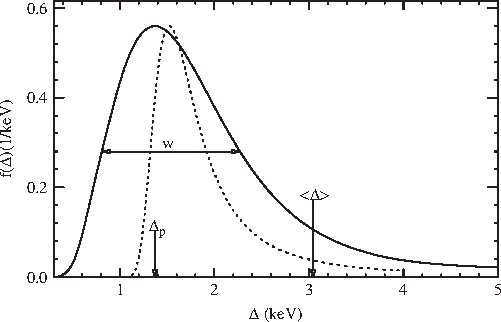
\includegraphics[width = 0.8\plotwidth]{fig/chapt4/Straggling-gas.pdf}\\
		\caption{\label{fig:straggling-gas} Example of straggling function $f(\Delta)$ of particles passing through \SI{1.2}{cm} of Argon gas with a $\beta\gamma$ of 3.6 and represented with a solid line. The original Landau distribution is showed with a dashed line~\cite{BISCHEL2006}.}
	\end{figure}
	
	\begin{figure}[H]
		\centering
		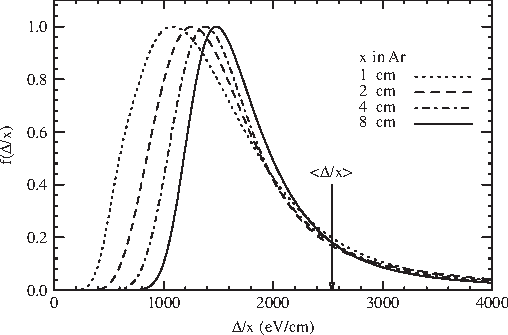
\includegraphics[width = 0.8\plotwidth]{fig/chapt4/Straggling-gas-thickness.pdf}\\
		\caption{\label{fig:straggling-thickness} Evolution of straggling functions $f(\Delta)$ of particles passing through a volume of Argon gas with a $\beta\gamma$ of 3.6 with increasing thickness $x$~\cite{BISCHEL2006}.}
	\end{figure}
	
	The mean energy loss per collision can be difficult to measure for low data samples and is not always representative of the energy loss distribution for a given incident particle energy. Hence, it is easier to access the most probable energy loss which is a lower value than than the average loss due to the distribution of the energy transfer. This value is well described by a highly skewed Landau distribution for detectors with "moderate" thickness $x$, expressed in \si{g.mol^{-1}}. But for gas volumes, a Landau distribution greatly underestimates the width $w$ of the distribution and only succeeds to provide with a correct value for the most probable energy loss, as showed in Figure~\ref{fig:straggling-gas}. Thus, the energy loss distribution is better represented by its most probable energy loss $\Delta_p$ and its \acf{FWHM} $w$. As showed by Figure~\ref{fig:straggling-thickness}, the distribution is affected by the thickness of the gas volume and the most probable energy loss normalized to the thickness is increased and the width decreased, converging towards the Landau distribution, whereas the mean energy loss is unchanged. Correction are brought to the original Landau equation in order to account better for the number of collisions leading to an increased width of the energy loss distribution~\cite{BISCHEL2006}.
	
	In the case of gas mixtures, composed of several elements, using Bragg additivity it can be understood that the mean energy loss of the mixture is the sum of the mean energy losses in each individual element $j$ layer of weight $w_j$.
	
	\begin{equation}
	\label{eq:mixtureloss}
	\left\langle \frac{dE}{dx} \right\rangle = \sum w_j \left\langle \frac{dE}{dx} \right\rangle_j
	\end{equation}
		
	\subsection{Primary ionization}
	\label{chapt4:ssec:ionization}
	
	Using Bethe formula to understand the mean energy transfer of charged particle when traveling through a gas volume give an intuition of the physics that affect the particle but doesn't provide a detailed enough information about the individual ionizations along its tracks at a microscopic level. In order to simulate efficiently an RPC and hence understand the processes  governing avalanches creation and growth, knowledge on the ionization process is necessary.
	
	To convert the energy loss rate into a number of primary ionizations was developed in 1980 the \acf{PAI} model~\cite{ALLISON1980} based on the cross section of ionization of gas atoms to real photons and the dielectric constant of the medium through which the charged particles are going. Indeed, the interaction of charged particles with the gas molecules being of electromagnetic nature, it is mediated by quasi-real photons and, hence, the cross section to photon ionization is important to understand. This approach is nevertheless semi-classical as it relies on classical electrodynamics and it only gives access to the energy transfer to the gas atoms and no information on the energy dissipation and secondary emissions is available on the output of the model. The energy transfered to the medium is not all used for ionization. For an energy deposition $\Delta$, the number of electron-ion pairs produced is:
	
	\begin{equation}
	\label{eq:npairs}
	\Delta = n_iW
	\end{equation}
	
	$W$ corresponds to the mean work per pair production that depends on the medium and is greater than the ionization potential leading to the conclusion that part of the transfered energy is dissipated through other processes~\cite{VINCENT2017,ICRU31}. In order to understand the energy dissipation and the secondary emissions, the fine structure of each atom is taken into account. Through the PAI model, the incident charged particle interacts is assumed to interact with the full atom rather than with a single electron.
	
	Although, considering that the particle interacts with a single electron, leads to the possibility to study the excited state of the atom once the photo-electron has been emitted with an energy corresponding to the transfered energy minus the binding energy of the electronic shell. The resulting vacancies in the electronic shell will be filled through emission of photons or Auger electrons and can contribute to further ionization or excitation in the gas volume. Fluorescence photons are usually not considered as they only constitute a very small fraction of secondary emissions~\cite{SMIRNOV2005}. Assuming that the transfered energy is absorbed in its totality by a single electronic shell, the PAI model was modified to include relaxations and constitute the new \acf{PAIR} model~\cite{SMIRNOV2005}. In this model, the cross section corresponding to the whole atom is re-expressed using a sum of partial cross sections corresponding to the different electronic shells. When one or more electrons are knocked out of the atom, the vacancies are filled by electrons of the shell above with relaxation by Auger electron emission. These processes happen in cascade from the inner shell to the outer one until all the vacancies are filled and the energy has been released.
	
	\begin{figure}[H]
		\begin{subfigure}{0.5\linewidth}
			\centering
			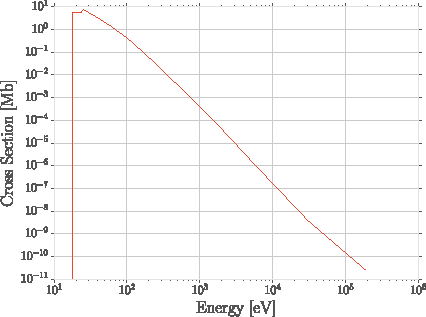
\includegraphics[width = 0.5\plotwidth]{fig/chapt4/HEED-Helium.pdf}
			\caption{\label{fig:PAIR:A} Helium}
		\end{subfigure}
		\begin{subfigure}{0.5\linewidth}
			\centering
			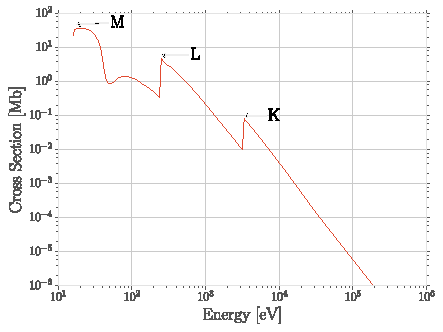
\includegraphics[width = 0.5\plotwidth]{fig/chapt4/HEED-Argon.pdf}
			\caption{\label{fig:PAIR:B} Argon}
		\end{subfigure}
		\begin{subfigure}{0.5\linewidth}
			\centering
			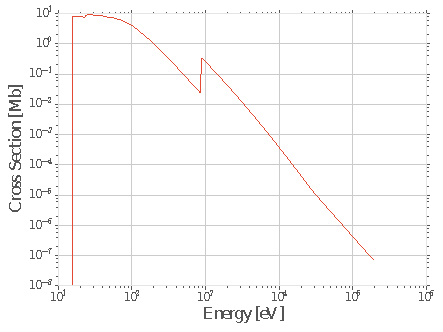
\includegraphics[width = 0.5\plotwidth]{fig/chapt4/HEED-Neon.pdf}
			\caption{\label{fig:PAIR:C} Neon}
		\end{subfigure}
		\begin{subfigure}{0.5\linewidth}
			\centering
			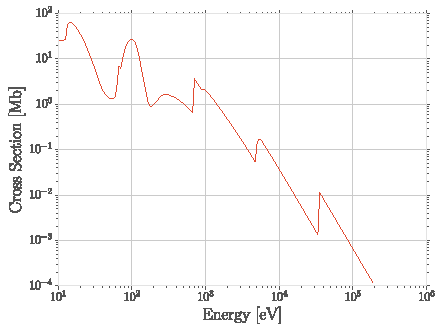
\includegraphics[width = 0.5\plotwidth]{fig/chapt4/HEED-Xenon.pdf}
			\caption{\label{fig:PAIR:D} Xenon}
		\end{subfigure}
		\caption{\label{fig:PAIR} Photo-absorption cross section as computed by \texttt{HEED} for nobles gases with different electric shell numbers~\cite{VINCENT2017}.}
	\end{figure}
	
	\begin{figure}[H]
		\centering
		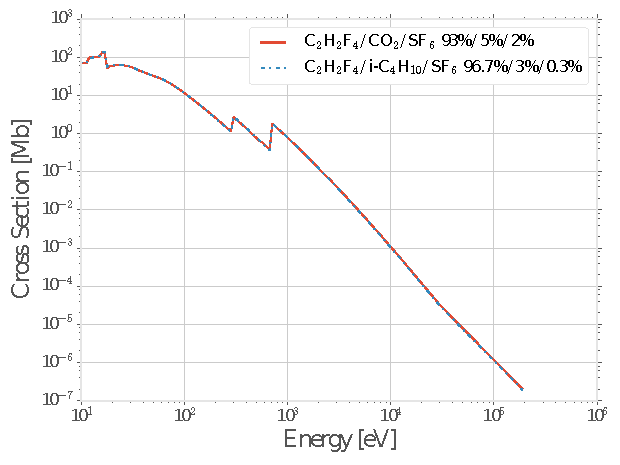
\includegraphics[width = 0.7\plotwidth]{fig/chapt4/HEED-RPC.pdf}\\
		\caption{\label{fig:PAIR-RPC} Photo-absorption cross section as computed by \texttt{HEED} for typical RPC gas mixtures~\cite{VINCENT2017}. The RPC mixture with $CO_2$ corresponds to the mixture used by CALICE SDHCAL~\cite{ARNAUD2015} while the other one was forseen for the experiement ATLAS~\cite{RIEGLER2003} but has been changed since then.}
	\end{figure}
	
	This model is included in the program \texttt{HEED} developed at CERN~\cite{HEED} and called by \texttt{Garfield}, a program developed for the simulation of gaseous detectors. The results for the cross section for a few noble gases are given in Figure~\ref{fig:PAIR}. It can be seen that for each shell, the cross section is increased. More complex patterns are seen with bigger atoms such as Xenon on Figure~\ref{fig:PAIR:D}. For gas mixtures, like the typical RPC mixtures, the cross section is showed in Figure~\ref{fig:PAIR-RPC}. Both mixtures being mainly composed of $C_2H_2F_4$, the variations in between the 2 cross section profiles are very subtle and depends on the concentration of the other compounds.
	
	\begin{figure}[H]
		\begin{subfigure}{\linewidth}
			\centering
			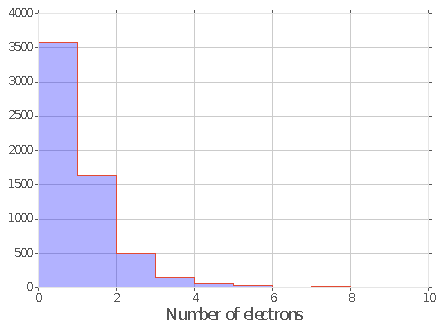
\includegraphics[width = 0.5\plotwidth]{fig/chapt4/N_elec_Helium.pdf}
			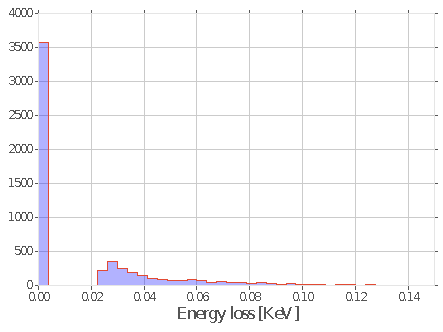
\includegraphics[width = 0.5\plotwidth]{fig/chapt4/E_loss_Helium.pdf}
			\caption{\label{fig:Primary:A} Helium}
		\end{subfigure}
		\begin{subfigure}{\linewidth}
			\centering
			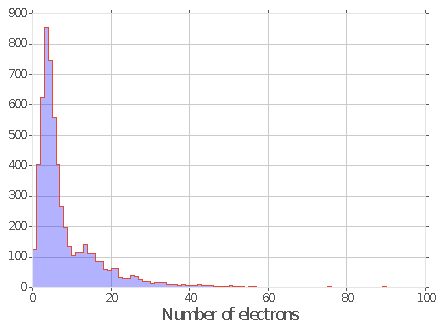
\includegraphics[width = 0.5\plotwidth]{fig/chapt4/N_elec_Argon.pdf}
			\includegraphics[width = 0.5\plotwidth]{fig/chapt4/E_loss_Argon.pdf}
			\caption{\label{fig:Primary:B} Argon}
		\end{subfigure}
		\begin{subfigure}{\linewidth}
			\centering
			\includegraphics[width = 0.5\plotwidth]{fig/chapt4/N_elec_RPC.pdf}
			\includegraphics[width = 0.5\plotwidth]{fig/chapt4/E_loss_RPC.pdf}
			\caption{\label{fig:Primary:C} 96.7\% $C_2H_2F_4$, 3\% i-$C_4H_{10}$ and 0.3\% $SF_6$~\cite{RIEGLER2003}}
		\end{subfigure}
		\caption{\label{fig:Primary} Distributions of number of electrons (left) and energy loss (right) for a \SI{5}{GeV/c} muon passing through \SI{1.2}{mm} of Helium (Figure~\ref{fig:Primary:A}), Argon (Figure~\ref{fig:Primary:B}) or a typical RPC gas mixture (Figure~\ref{fig:Primary:C})~\cite{VINCENT2017}.}
	\end{figure}
	
	Once the cross section of interaction is known, it is possible to extract the distribution of energy loss and of the number of electron produced, as showed in Figure~\ref{fig:Primary} for Helium, Argon, which is used in gaseous detectors, and for a typical RPC mixture~\cite{VINCENT2017}. The distributions are computed using \texttt{HEED} and show typical straggling function profiles with some complex structures that can be related to interaction of the incoming particle with the different electronic shells. Helium does not have a great photo-absorption cross-section according to Figure~\ref{fig:PAIR:A} and a muon will not be likely to lose a lot of energy and to create a lot of electrons whereas in a more complex atom like Argon, the cross-section is greater and will lead to a greater energy loss of muons and more electron produced. Finally, a complex gas mixture used in RPCs will offer an even greater cross-section, a wider energy loss distribution and will be able to produce more electrons. The same information is seen by looking at the evolution of the mean number of cluster as a function of the lorentz factor associated to muons showed in Figure~\ref{fig:ClusterDensity:A}. Indeed, the greater photo-absorption cross-section of RPC mixtures allow for a much greater amount of clusters to be created by charged particles. The size of these clusters is studied through Figure~\ref{fig:ClusterDensity:B} which shows that, in most of the cases ($\approx$80\%), the clusters only are composed of a single electron which is consistent with minimum ionizing particles.
	
	\begin{figure}[H]
		\begin{subfigure}{0.5\linewidth}
			\centering
			\includegraphics[width = 0.5\plotwidth]{fig/chapt4/Cluster-distribution.pdf}
			\caption{\label{fig:ClusterDensity:A}}
		\end{subfigure}
		\begin{subfigure}{0.5\linewidth}
			\centering
			\includegraphics[width = 0.5\plotwidth]{fig/chapt4/N_elec_cluster_RPC.pdf}
			\caption{\label{fig:ClusterDensity:B}}
		\end{subfigure}
		\caption{\label{fig:ClusterDensity} Figure~\ref{fig:ClusterDensity:A}: Mean cluster density for muons through different gas volumes~\cite{VINCENT2017}. Figure~\ref{fig:ClusterDensity:B}: Distribution of the number of electrons per cluster for a \SI{5}{GeV/c} muon traveling through a mixture of 96.7\% $C_2H_2F_4$, 3\% i-$C_4H_{10}$ and 0.3\% $SF_6$~\cite{VINCENT2017,RIEGLER2003}.}
	\end{figure}
	
	\subsection{Development and propagation of avalanches}
	\label{chapt4:ssec:avalanche}
	
	From the clusters released in the gas volume by the charged particles, free electrons will start drifting due to the electric applied in between the electrodes of the RPC. Gaining velocity and energy, these electrons in their turn will be able to ionize the gas. This process being repeated by all the produced electrons will trigger an avalanche to develop.
	
	The growth of the avalanche can be intuitively understood as a competition between 2 effects. Due to their increasing energy, electrons have a probability to trigger new ionizations by interacting with gas molecules. On the other hand, before the minimal amount of energy is reached, the electrons can get attached to a gas molecule instead. These two effects can be described using a simple model in which the multiplication and attachment processes are given by the Townsend coefficient $\alpha$ and the attachment coefficient $\eta$, assuming that the history of previous interactions in the gas does not influence new interactions. This model simply takes into account probabilities to have at the gas depth $z$ for a given number $n$ of free electrons in the gas $n+1$ or $n-1$ electrons  at the depth $z+\deriv z$ (respectively $n\alpha\deriv z$ and $n\eta\deriv z$). Then, the mean number of electrons $\bar{n}$ and cations $\bar{p}$ can be written for single compound gases as
	
	\begin{equation}
	\label{eq:townsend}
	\frac{\deriv\bar{n}}{\deriv z} = (\alpha - \eta)\bar{n} \, , \;\;\;\; \frac{\deriv\bar{p}}{\deriv z} = \alpha\bar{n}
	\end{equation}
	
	which, assuming the initial conditions $\bar{n}(0) = 1$ and $\bar{p}(0) = 0$, lead to the mean number of electrons and cations at a depth $z$
	
	\begin{equation}
	\label{eq:Townsend-avalanche}
	\bar{n}(z) = e^{(\alpha - \eta)z} \, , \; \bar{p}(z) = \frac{\alpha}{\alpha - \eta}\left( e^{(\alpha - \eta)z} - 1\right)
	\end{equation}
	
	The Townsend and attachment coefficient as a function of the applied electric field are given in Figure~\ref{fig:Townsend} for a standard RPC gas mixture using \texttt{Magboltz}~\cite{MAGBOLTZ}.
	
	\begin{figure}[H]
		\centering
		\includegraphics[width = 0.7\plotwidth]{fig/chapt4/Townsend-RPC.pdf}\\
		\caption{\label{fig:Townsend} Townsend and attachment coefficient for a typical 96.7/3/0.3 mixture of $C_2H_2F_4$/i-$C_4H_{10}$/$SF_6$, at a temperature $T=$\SI{296.15}{K} and a pressure $P=$\SI{1013}{hPa}~\cite{VINCENT2017,RIEGLER2003}.}
	\end{figure}
	
	Nevertheless, there are more to the avalanche growth than simply these two factors. Throughout the \Th{20} century, models have been developed to better understand the physics of discharges in gas. In 1937, Furry developed a model to describe electromagnetic cascades~\cite{FURRY1937} that would be used for electron avalanches in gas during the 1950s. Furry realized that the use of a Poisson law to describe the distribution of shower sizes could not be accurate as he understood that the events occurring in the development of a cascade are not independent from each other, as a Poisson law would suggest. Indeed, part of the particles produce others and this process depends on both their original energy and energy lost. Experimental results showed excess of small showers and an under estimate of very large ones. To solve this problem, Furry proposed a distribution of sizes of following the likelihood described in Equation~\ref{eq:Furry}, in which $\bar{n} = e^{\alpha z}$, compared with a Poisson law in Figure~\ref{fig:furry}.
	
	\begin{equation}
	\label{eq:Furry}
	P(n,\bar{n}) = \bar{n}^{-1} (1-\bar{n}^{-1})^{n-1}
	\end{equation}
	
	\begin{figure}[H]
		\centering
		\includegraphics[width = 0.7\plotwidth]{fig/chapt4/Furry.png}\\
		\caption{\label{fig:furry} Comparison of the distribution law of Furry and the Poisson law for $\bar{n} = 5$~\cite{FURRY1937}.}
	\end{figure}
	
	\begin{figure}[H]
		\centering
		\includegraphics[width = 0.6\plotwidth]{fig/chapt4/Genz1973.png}\\
		\caption{\label{fig:genz} Single-electron avalanche size distribution in a proportionnal counter filled with methylal at different $E/p$ values. (a) 70, (b) 76.5, (c) 105, (d) 186.5, (e) 426\si{V/cm.torr}~\cite{GENZ1973}.}
	\end{figure}
	
	In this model, no extra energy is brought to the electrons in the showers, contrary to the case of a gaseous detector such as a RPC where an electric field accelerates them. Using the Furry model, Genz studied the fluctuations in electron avalanches in gaseous detectors~\cite{GENZ1973}. Collisions leading to ionizations leave electrons with an energy much smaller than the ionization energy $eU_i$, where $U_i$ is the ionization potential of a gas molecule. Hence, the electrons need to travel a distance $s = U_i/E$ along the electric field $E$ to acquire a high enough energy to trigger a new ionization. For the probability of a new ionization to be independent from the path followed by the electrons since the previous ionization, the mean free path $1/\alpha$ of electrons in the gas has to be large compared to $s$ and thus $E/\alpha \gg U_i$. The Townsend coefficient is related to the gas pressure leading to conditions on the value of $E/p$. Avalanches in gas are large compared to the showers Furry has studied in his original paper. For very large avalanche sizes, Equation~\ref{eq:Furry} can be written as an exponential, as showed in Equation~\ref{eq:FurryGenz}.
	
	\begin{equation}
	\label{eq:FurryGenz}
	P(n,\bar{n}) = \bar{n}^{-1} e^{-n/\bar{n}}
	\end{equation}
	
	This exponential behaviour is showed through Figure~\ref{fig:genz}. In practice, to fully understand the avalanche growth, taking into account the path followed by electrons from one ionization to another will become necessary. In the same paper, Genz then discusses models using Polya distributions to estimate the multiplication by looking at the size of the avalanche it self. Indeed, the number of charge carriers in the avalanche might become important enough to have an effect on the multiplication process. To account for this, it was proposed to use a varying Townsend coefficient such as described by Equation~\ref{eq:Polya-T} depending on the position $x$ in which $\theta$ is an empirical parameter leading to the probability distribution of Equation~\ref{eq:Polya-P}. In the limit case where $\theta$ goes to 0, the formula describes again the Furry model. But the data deviates from this model as well at large n values. Moreover, the introduction of an empirical parameters makes the model hard to interpret physically.
	
	\begin{equation}
	\label{eq:Polya-T}
	\alpha(n,x) = \alpha(x) \left( 1 + \frac{\theta}{n} \right) \, , \;\;\;\; n > 0
	\end{equation}
	
	\begin{equation}
	\label{eq:Polya-P}
	P(n,x) = \frac{1+\theta}{\bar{n}}\frac{1}{\theta !} \left( \frac{n(1+\theta)}{\bar{n}} \right)^\theta e^{-\frac{n(1+\theta)}{\bar{n}}}
	\end{equation}
	
	In order to have a model that describes reality better, the introduction of the attachment into the model is an important step. Despite its limitations, the Furry model had the advantage to describe well avalanches occurring when the attachment could be ignored. This is only natural that this model was then extended to included attachment. This was done by Riegler, Lippmann and Veenhof~\cite{RIEGLER2003} which showed that was important was to consider both the Townsend coefficient describing the multiplication \textit{and} the attachment coefficient, not only the effective multiplication coefficient $\bar{\alpha} = \alpha - \eta$. The probability to see an avalanche started by a single electron grow to a size $n$ after having traveled a distance $z$ through the gas is given by Equation~\ref{eq:RLV}.
	
	\begin{equation}
	\label{eq:RLV}
		\begin{aligned}
		P(n,z) &= P(n-1,z) \, (n-1)\alpha\deriv{z} \, (1-(n-1)\eta\deriv{z})\\
			   &+ P(n,z)   \, (1-n\alpha\deriv{z}) \, (1-n\eta\deriv{z})\\
			   &+ P(n,z)   \, n\alpha\deriv{z} \, n\eta\deriv{z}\\
			   &+ P(n+1,z) \, (1-(n+1)\alpha\deriv{z}) \, (n+1)\eta\deriv{z}
		\end{aligned}
	\end{equation}
	
	The first term of this probability that from a state with $n-1$ electrons, only 1 multiplies while the others don't get attached. Both the second and third terms describes the probability that from a state with already $n$ electrons the total number of electrons stay the same. On the second term, no electron gets attached nor multiplies while on the third term, 1 electron gets multiplied and 1 gets attached to compensate. Finally, the fourth term describes the probability to fall from a state with $n+1$ to a state with $n$ electrons due to the attachment of a single electron. At the first order, the evaluation of the previous expression leads to Equation~\ref{eq:dRLV} which general solution is given in Equation~\ref{eq:sol-RLV} in which are introduced the variables $\bar{n}(z)$, defined as in Equation~\ref{eq:Townsend-avalanche}, and $k = \eta/\alpha$ making explicit the fact that the distribution not only depends on the effective Townsend coefficient.
	
	\begin{equation}
	\label{eq:dRLV}
	\frac{\deriv{P(n,z)}}{\deriv{z}} = -P(n,z)n(\alpha+\eta) \, + \, P(n-1,z)(n-1)\alpha \, + \, P(n+1,z)(n+1)\eta
	\end{equation}
	
	\begin{equation}
	\label{eq:sol-RLV}
	P(n,z) = \left\{
				\begin{array}{l l}
  				k\frac{\bar{n}(z)-1}{\bar{n}(z)-k} \, , & n=0\\
  				\bar{n}(z) \left( \frac{1-k}{\bar{n}(z)-k} \right)^2 \left( \frac{\bar{n}(z)-1}{\bar{n}(z)-k} \right)^{n-1} \, , & n>0\\
  				\end{array} \right.
	\end{equation}
	
	The example given through Figure~\ref{fig:RVL} shows the importance of each individual process in the growth of avalanches and the fluctuation of their size. The values of $\alpha$ and $\eta$ will influence the probability distribution, as can be seen from Figure~\ref{fig:RVL:A}. Then, Figure~\ref{fig:RVL:B} shows that the fluctuation really takes place within the very first interactions. Indeed, when the avalanche contains a large enough amount of charge carriers (a few hundreds), its size then increases like $e^{z(\alpha-\eta)}$.
	
	\begin{figure}[H]
		\begin{subfigure}{0.5\linewidth}
			\centering
			\includegraphics[width = 0.5\plotwidth]{fig/chapt4/Riegler-distrib.pdf}
			\caption{\label{fig:RVL:A}}
		\end{subfigure}
		\begin{subfigure}{0.5\linewidth}
			\centering
			\includegraphics[width = 0.5\plotwidth]{fig/chapt4/Riegler-fluctuations.pdf}
			\caption{\label{fig:RVL:B}}
		\end{subfigure}
		\caption{\label{fig:RVL} Figure~\ref{fig:RVL:A}: Comparison of avalanche size distributions for different values of Townsend and attachment coefficients. The effective Townsend coefficient is the same for both distributions. Figure~\ref{fig:RVL:B}: Fluctuation in avalanche size for avalanche started by a single electron with $\alpha$ = \SI{13}{mm^{-1}} and $\eta$ = \SI{3.5}{mm^{-1}}~\cite{RIEGLER2003}.}
	\end{figure}
		
	\subsection{Drift and diffusion of the electron cloud}
	\label{chapt4:ssec:electrons}
	
	During the growth of avalanches, an electron cloud drifting along the electric field through the gas will undergo thermal diffusion due to random collisions with the gas molecules. This phenomenon can be studied using Maxwell-Boltzmann distribution whose mean is defined by the thermal energy of the cloud $\left\langle E\right\rangle = 3/2 kT$ with an extra component coming from the constant drift motion. The drift of electrons along the field lines is usually observed on a macroscopic scale through which the speed can be assimilated to a constant $v_D$ which corresponds to the mean drift speed over a large number of collisions in the gas.
	
	\begin{figure}[H]
		\begin{subfigure}{\linewidth}
			\centering
			\includegraphics[width = 0.6\plotwidth]{fig/chapt4/Drift_velocity.pdf}
			\caption{\label{fig:Drift-Diff:A}}
		\end{subfigure}
		\begin{subfigure}{0.5\linewidth}
			\centering
			\includegraphics[width = 0.55\plotwidth]{fig/chapt4/Diff_Trans.pdf}
			\caption{\label{fig:Drift-Diff:B}}
		\end{subfigure}
		\begin{subfigure}{0.5\linewidth}
			\centering
			\includegraphics[width = 0.55\plotwidth]{fig/chapt4/Diff_Long.pdf}
			\caption{\label{fig:Drift-Diff:C}}
		\end{subfigure}
		\caption{\label{fig:Drift-Diff} Figure~\ref{fig:Drift-Diff:A}: Electron mean drift velocity $v_D$ in pure $C_2H_2F_4$ and typical RPC gas mixtures. Figure~\ref{fig:Drift-Diff:B}: Transverse diffusion coefficient in pure $C_2H_2F_4$ and a typical RPC gas mixture. Figure~\ref{fig:Drift-Diff:C}: Longitudinal diffusion coefficient in pure $C_2H_2F_4$ and a typical RPC gas mixture. All results are given with a pressure $P = $ \SI{760}{Torr} and a temperature $T =$ \SI{296.15}{K}~\cite{VINCENT2017}.}
	\end{figure}
	
	\begin{figure}[H]
		\begin{subfigure}{0.5\linewidth}
			\centering
			\includegraphics[width = 0.55\plotwidth]{fig/chapt4/Elec_distrib_no_diff.pdf}
			\caption{\label{fig:Diff-Distrib:A} $n_e =$ \Sci{4.01}{5}}
		\end{subfigure}
		\begin{subfigure}{0.5\linewidth}
			\centering
			\includegraphics[width = 0.55\plotwidth]{fig/chapt4/Elec_distrib_w_diff.pdf}
			\caption{\label{fig:Diff-Distrib:B} $n_e =$ \Sci{1.25}{6}}
		\end{subfigure}
		\caption{\label{fig:Diff-Distrib} Comparison of the free charge carriers in the gas after a time $t =$ \SI{7.90}{ns} in the case where no diffusion is taken into account to simulate the avalanche (Figure~\ref{fig:Diff-Distrib:A}) and in the case where the diffusion is implemented (Figure~\ref{fig:Diff-Distrib:B})~\cite{VINCENT2017}.}
	\end{figure}
	
	Indeed, at the microscopic scale, the electrons are drifting over a distance $\delta z$ while acquiring the corresponding kinetic energy $T = e_0 \vert\overrightarrow{E}\vert\delta z$ until they are slowed down by a collision in which they lose part of their energy. This process is repeated as long as electrons are free carriers. Starting from a point-like electron cloud, the Gaussian density distribution at $\overrightarrow{r_0}$ will be described by Formula~\ref{eq:Diff-Gauss} in which the width of the isotropic distribution is $\sigma = 2\bar{D}t$, with $\bar{D}$ being a diffusion coefficient expressed in \si{m^2/s}~\cite{LIPPMANN2003}.
	
	\begin{equation}
	\label{eq:Diff-Gauss}
	\varphi(\overrightarrow{r},t) = \frac{1}{\left(\sqrt{2\pi}\sigma(t)\right)^3} exp\left( -\frac{(\overrightarrow{r} - \overrightarrow{r_0})^2}{2\sigma^2(t)} \right)
	\end{equation}
	
	Now, if the constant drifting motion is added, the distribution is anisotropic and can be divided onto transversal (Formula~\ref{eq:Diff-Trans}) and longitudinal (Formula~\ref{eq:Diff-Long}) terms, $\varphi(r,z,t) = \varphi_T(r,t)\varphi_L(z,t)$, with a cylindrical symmetry around the field axis~\cite{LIPPMANN2003}. The variables $t$ and $\sigma_{T,L}(t)$ can be hidden to the profit of the diffusion coefficients by using the relations $v_D = l/t$ and $\sigma_{T,L}^2(t) = 2\bar{D}_{T,L}l/v_D$ and introducing new diffusion coefficients $D_{T,L} = \sqrt{2\bar{D}_{T,L}/v_D}$ in order to explicitly show the dependence of the Gaussian width in drifted distance $l$.
	
	\begin{equation}
	\label{eq:Diff-Trans}
	\varphi_T(r,t) = \frac{1}{D_T^2l} exp\left( -\frac{(r - r_0)^2}{2D_T^2l} \right)
	\end{equation}
	
	\begin{equation}
	\label{eq:Diff-Long}
	\varphi_L(z,t) = \frac{1}{\sqrt{2\pi l}D_L} exp\left( -\frac{(z - z_0)^2}{2D_L^2l)} \right)
	\end{equation}
	
	These coefficients, as well as the drift velocity of the electrons, can be calculated thanks to \texttt{Magboltz} as showed in Figure~\ref{fig:Drift-Diff}. The influence of the diffusion on the distribution of charge carriers throughout the gas volume is depicted in Figure~\ref{fig:Diff-Distrib}. From very localised electron clusters in the gas in Figure~\ref{fig:Diff-Distrib:A}, a Gaussian diffusion is then visible in Figure~\ref{fig:Diff-Distrib:B}. Due to the interactions with gas molecules during the drift, diffusions can occur in the forward and backward direction. Electrons diffused backward will effectively drift over a longer distance and multiply more than electrons diffused forward that will see a shorter drift length. As an effect, the avalanche develops over a longer time and extends over a greater gas volume than in the case the electron cloud is considered as point like and without diffusion. Moreover, as a side effect to the longer growth of the avalanche due to backward longitudinal diffusion, the total production of electrons is increased.
	
	\subsection{Space charge effect \& streamers}
	\label{chapt4:ssec:space-charge}
	
	Now that have been considered the basic processes that influence the development of avalanches in a gaseous detector in the previous sections, it is now important to consider the influence of the charge carriers present in the avalanche on the electric field seen by the avalanche. Indeed, each charged particle induces an electric field and it is only natural that the increasing density of electrons and ions in the detector volume will affect the electric field. Thus, parameters such as the Townsend and attachment coefficients, drift velocity or diffusion coefficients will find themselves to be modified along the gas gap length due to this effect referred to as \textit{space charge effect}. Figure~\ref{fig:Space_charge} is a more detailed version of Figure~\ref{fig:RPC_principle} \textit{(b)} in which three electric regions are distinguished~\cite{LIPPMANN2003}. When compared to the linear electric field of strength $E_0$ that is developed in between the detector's electrodes, the accumulation of negative charges (electrons) on the front of the avalanche will reinforce the effective electric field in between the anode of the avalanche front. Deeper in the gas volume, the positive charges (cations) slowly drift towards the cathode and can induce together with the avalanche front opposite electric field loops. Finally, due to the density of positive charges, the electric field seen in between the ions tails and the cathode charged with negative charges is on average stronger than $E_0$ and compensate for the locally reversed field $E_2$. Lippmann roughly estimated by considering that \Ord{6} charges were contained in a sphere of radius $r_d =$ \SI{0.1}{mm} that the space charge effect could change the electric field by 3\% and the Townsend and attachment coefficient up to 14\%~\cite{LIPPMANN2003,VINCENT2017}.
	
	\begin{figure}[H]
		\centering
		\includegraphics[width = 0.7\plotwidth]{fig/chapt4/Avalanche_space_charge.pdf}\\
		\caption{\label{fig:Space_charge} Schematic representation of an avalanche and of the electric field deformation it causes due to the local concentration of charge carriers~\cite{LIPPMANN2003}.}
	\end{figure}
	
	To account for the space charge effect, the electric potential and field of free charges are solved and applied to each charges in the avalanche~\cite{LIPPMANN2003,VINCENT2017}. As discussed by Français who has been working on simulating RPCs similar to that used by the SDHCAL project of ILC, the computation of these equations for each individual charge carrier to dynamically know the space charge field at every stage of an avalanche development is a difficult task and would require far too much computation time and a solution is to pre-compute an interpolation table keeping an adequately large number of values of the space charge field for each positions in space thanks to which the values stored in the interpolation table become very close to the analytic solution and allow for a much faster simulation.\\
	
	The study of space charge effect through simulation shows that the it can lead to a saturation of the avalanche growth due to the deformation of the electric field, as showed through Figure~\ref{fig:Space-charge-effect}. Additionnally, a more precise understanding of the space charge effect is given through Figure~\ref{fig:Avalanche-develop} which looks at the distribution of charges and the distortion of the electric field at different steps of the evolution of an avalanche in a RPC. At the moment a \SI{5}{GeV} muon ionizes the gas, electron-ion pairs are created in the gas in different clusters (Figure~\ref{fig:Avalanche-develop:A}). Later, the first clusters have reached the anode while the clusters that where created the closest to the cathode are now big enough to start influencing the electric field in the gap (Figure~\ref{fig:Avalanche-develop:B}). When a cluster is big enough, the electric field in front of it locally increases a lot and contributes to a stronger but very localised multiplication. At the same moment, the positive ions right behind the cluster avalanche front decrease the electric field, saturating the electron multiplication on the tail of the electron cloud (Figure~\ref{fig:Avalanche-develop:C}). Finally, when all the electrons have reached the anode and are relaxing, the electric field still is very deformed by the distribution of both positive and negative ions in the the gas volume closest to the anode (Figure~\ref{fig:Avalanche-develop:D}).
	
	\begin{figure}[H]
		\begin{subfigure}{0.5\linewidth}
			\centering
			\includegraphics[width = 0.55\plotwidth]{fig/chapt4/Induced_charge_no_space_charge.pdf}
			\caption{\label{fig:Space-charge-effect:A}}
		\end{subfigure}
		\begin{subfigure}{0.5\linewidth}
			\centering
			\includegraphics[width = 0.55\plotwidth]{fig/chapt4/Induced_charge_w_space_charge.pdf}
			\caption{\label{fig:Space-charge-effect:B}}
		\end{subfigure}
		\caption{\label{fig:Space-charge-effect} Evolution of the charge induced by an avalanche started by a single electron in a \SI{1.2}{mm} thick RPC with an applied electric field of \SI{54}{kV/cm} in the case space charge is not taken into account (Figure~\ref{fig:Space-charge-effect:A}) and in the case it is implemented into the simulation (Figure~\ref{fig:Space-charge-effect:B}). The total induced charge is correlated to the size of the avalanche~\cite{VINCENT2017}.}
	\end{figure}
	
	\begin{figure}[H]
		\begin{subfigure}{0.5\linewidth}
			\centering
			\includegraphics[width = 0.55\plotwidth]{fig/chapt4/Avalanche_dev_step1.pdf}
			\caption{\label{fig:Avalanche-develop:A} $t=$ \SI{0}{ns}}
		\end{subfigure}
		\begin{subfigure}{0.5\linewidth}
			\centering
			\includegraphics[width = 0.55\plotwidth]{fig/chapt4/Avalanche_dev_step2.pdf}
			\caption{\label{fig:Avalanche-develop:B}$t=$ \SI{7.94}{ns}}
		\end{subfigure}
		\begin{subfigure}{0.5\linewidth}
			\centering
			\includegraphics[width = 0.55\plotwidth]{fig/chapt4/Avalanche_dev_step3.pdf}
			\caption{\label{fig:Avalanche-develop:C}$t=$ \SI{8.94}{ns}}
		\end{subfigure}
		\begin{subfigure}{0.5\linewidth}
			\centering
			\includegraphics[width = 0.55\plotwidth]{fig/chapt4/Avalanche_dev_step4.pdf}
			\caption{\label{fig:Avalanche-develop:D}$t=$ \SI{23.9}{ns}}
		\end{subfigure}
		\caption{\label{fig:Avalanche-develop} Distributions of charge carriers within the gas volume of a \SI{1.2}{mm} thick RPC and the corresponding deformation of the electric field at different time steps with an applied electric field of \SI{55.5}{kV/cm}~\cite{VINCENT2017}.}
	\end{figure}
	
	The electric field following the development of an avalanche can stay perturbed for a long time with respect to the avalanche development due to the slow drift of the much heavier ions. This can result in powerful secondary avalanches triggered by the fluctuation of the electric field together with the emission of UV-photons leading to emission of electrons at the surface of the electrode. This is a slow phenomenon compared to the development of avalanches. Experimentally, it is observed that the stronger the electric field applied over the gap, the sooner after the avalanche, referred to as \textit{precursor signal} in this context, and the stronger will the secondary avalanche be, possibly reaching the streamer regime. This could be due to the amount of UV-photons emitted by the growing precursor. These photons will be able to trigger new avalanches in a radius of a few \si{mm} around the precursor by knocking electrons from the cathode by photoelectric effect. The strong distortions of the electric field due to a large avalanche will be more likely to emit UV-photons as the electric field at the front of the precursor avalanche will be large, providing the electrons with a larger energy. Eventually, the new avalanches can grow to form streamers.
	
\section{Effect of atmospherical conditions on the detector's performance}
\label{chapt4:sec:PTcorrection}
	
	\begin{figure}[H]
		\centering
		\includegraphics[width = 0.7\plotwidth]{fig/chapt4/Weighting_field.pdf}\\
		\caption{\label{fig:weighting-field} Representation of the weighting field in the volume of a RPC and the resulting induced current in the strip placed at \SI{1}{V} and its neighbour connected to the ground. The induced current corresponds, as can be understood from Formula~\ref{eq:IndCurrent}~\cite{LIPPMANN2003}.}
	\end{figure}

	Accordingly to Ramo's theorem, the movement of charge carriers, and in particular, the movement of a dense electron cloud toward the anode induces a current signal on one or more of the readout electrodes (strips or pads). The ions on the other hand induce only a very small current as their movement is much slower than which of the electrons. The current induced by $n_Cl$ clusters of $N_j(t)$ charge carriers drifting at velocities $\overrightarrow{v_{Dj}}(t) = \dot{\overrightarrow{x_j}}(t)$ at a time $t$ is given by Formula~\ref{eq:IndCurrent} in which $e_0$ is the unit charge and $\overrightarrow{E_w}$ is the \textit{weighting field}.
	
	\begin{equation}
	\label{eq:IndCurrent}
	i(t) = \sum_{j=1}^{n_Cl} \overrightarrow{E_{wj}}(\overrightarrow{x_j}(t)) \cdot \overrightarrow{v_{Dj}}(t) e_0 N_j(t)
	\end{equation}
	
	The weighting field, that has been schematised in Figure~\ref{fig:weighting-field}, corresponds to the electric field that would be oberved in the gas gap if a readout electrode is placed at a potential of \SI{1}{V} while keeping all the other electrodes grounded. Then the induced charge in the readout can be simply obtained by integrating Formula~\ref{eq:IndCurrent} over the duration $T$ of the signal, as given by Formula~\ref{eq:IndCharge}.
	
	\begin{equation}
	\label{eq:IndCharge}
	Q(t) = \int_0^T \sum_{j=1}^{n_Cl} \overrightarrow{E_{wj}}(\overrightarrow{x_j}(t)) \cdot \overrightarrow{v_{Dj}}(t) e_0 N_j(t)
	\end{equation}
	
	The signal induced in the readout of RPCs operated in avalanche mode is then sent into \acl{FEE} in which they will be pre-amplified and discriminated. The discrimination and digitization of signals in CMS FEE is described through Figure~\ref{fig:CMS-FEE}. On a first stage, analogic signals are amplified, following the curve given on Figure~\ref{fig:CMS-FEE-preamp}, and then sent to the \acf{CFD} described in Figure~\ref{fig:CFD}. At the end of the chain, \SI{100}{ns} long pulses are sent in the LVDS output. The digital signals are both used as trigger for CMS and to evaluate the performance of the detectors. The performance will dependent on the applied HV, i.e. on the electric field inside of the gas volume, but also on the threshold applied on the CFDs. Indeed, in order to reduce the probability to measure noise, the threshold is set to a level where the noise is strongly suppressed while the signals are not too affected. Typically, CMS FEEs are set to a threshold of \SI{215}{mV} after pre-amplification, corresponding to an input charge of about \SI{140}{fC}.
	
	\begin{figure}[H]
		\centering
		\includegraphics[width = 0.6\plotwidth]{fig/chapt4/CMS-FEE.pdf}\\
		\caption{\label{fig:CMS-FEE} Schematics of CMS RPC FEE logic.}
	\end{figure}
	
	\begin{figure}[H]
		\centering
		\includegraphics[width = 0.7\plotwidth]{fig/chapt4/CMS-FEE-preamp.pdf}\\
		\caption{\label{fig:CMS-FEE-preamp} Equivalence in between the charge of the induced signal in input of the CMS FEE and the signal strength on the output of the pre-amplier.}
	\end{figure}
	
	\begin{figure}[H]
		\begin{subfigure}{\linewidth}
			\centering
			\includegraphics[width = 0.7\plotwidth]{fig/chapt4/CFD_1.pdf}\\
			\caption{\label{fig:CFD:A}}
		\end{subfigure}
		\begin{subfigure}{\linewidth}
		    \centering
			\includegraphics[width = 0.84\plotwidth]{fig/chapt4/CFD_2.png}
			\caption{\label{fig:CFD:B}}
		\end{subfigure}
		\caption{\label{fig:CFD} Description of the principle of a CFD. A comparison of threshold triggering (left) and constant franction triggering (right) is shown in Figure~\ref{fig:CFD:A}. Constant franction triggering is obtained thanks to zero-crossing technique as explained in Figure~\ref{fig:CFD:B}. The signal arriving at the input of the CFD is split into three components. A first one is delayed and connected to the inverting input of a first comparator. A second component is connected to the noninverting input of this first comparator. A third component is connected to the noninverting input of another comparator along with a threshold value connected to the inverting input. Finally, the output of both comparators is fed through an AND gate.}
	\end{figure}
	
	The performance of a detector is then simply measured relatively to which of a reference detector used as trigger as the ratio in between the number of events recorded in coincidence in the detector and the reference and the total amount of trigger events, $\epsilon = n_{events}/n_{triggers}$. An example of efficiency measured as a function of the effective voltage $HV_{eff}$ is given in Figure~\ref{fig:Sigmoid} and can be fitted thanks to a sigmoidal function described as in Formula~\ref{eq:Sigmoid} and where $\epsilon_{max}$ is the maximal efficiency of the detector, $\lambda$ is proportional to the slope at half maximum and $HV_{50}$ is the value of the voltage when the efficiency reaches half of the maximum.
	
	\begin{equation}
	\label{eq:Sigmoid}
	\epsilon(HV_{eff}) = \frac{\epsilon_{max}}{1+e^{-\lambda(HV_{eff}-HV_{50})}}
	\end{equation}
	
	CMS RPC also define two points on this sigmoid that called \textit{knee} and \textit{working point}. The corresponding voltages $HV_{knee}$ is defined as the voltage at 95\% of the maximum efficiency, and $HV_{WP}$ is defined as in Formula~\ref{eq:KneeWP}.
	
	\begin{equation}
	\label{eq:KneeWP}
	HV_{WP} = HV_{knee} + \left\{\begin{array}{l l}100\mathrm{V} & \quad \mathrm{(barrel)}\\ 150\mathrm{V} & \quad \mathrm{(endcap)}\\ \end{array}\right.
	\end{equation}
	
	\begin{figure}[H]
		\centering
		\includegraphics[width = 0.7\plotwidth]{fig/chapt4/Eff_sigmoid.png}\\
		\caption{\label{fig:Sigmoid} Typical efficiency sigmoid of a CMS RPC detector. The black dots correspond to the data, the blue line to the sigmoid fit and the opened cross to the knee and working extracted from the fit line.}
	\end{figure}
	
	Nevertheless, the voltage applied on a detector may vary due to a change in environmental conditions. Indeed, the variation of temperature and/or pressure will have effects on the gas density and the electrodes' resistivity which can be overcome by changing the electric field accordingly. The variation in temperature and pressure are depicted respectively in Figure~\ref{fig:TCorr} and Figure~\ref{fig:PCorr}. A standard procedure to correct for temperature and pressure variations is to keep the factor $HV\cdot T/P$ constant using Formula~\ref{eq:PTSimple}~\cite{ABBRESCIA1995,ABBRESCIA1997PRES} with reference values for $T_0$ and $P_0$. For example, CMS uses $T_0=$ \SI{293.15}{K} and $P_0=$ \SI{965}{hPa}.
	
	\begin{equation}
	\label{eq:PTSimple}
	HV_{app} = HV_{eff}\frac{P_0}{P}\frac{T}{T_0}
	\end{equation}
	
	\begin{figure}[H]
		\begin{subfigure}{0.5\linewidth}
			\centering
			\includegraphics[width = 0.58\plotwidth]{fig/chapt4/Rate-temperature.png}\\
			\caption{\label{fig:TCorr:A}}
		\end{subfigure}
		\begin{subfigure}{0.5\linewidth}
		    \centering
			\includegraphics[width = 0.58\plotwidth]{fig/chapt4/Efficiency-temperature.png}
			\caption{\label{fig:TCorr:B}}
		\end{subfigure}
		\caption{\label{fig:TCorr} Effect of the temperature variation on the rate (Figure~\ref{fig:TCorr:A}) and the efficiency (Figure~\ref{fig:TCorr:B}) of a RPC~\cite{ABBRESCIA1995}.}
	\end{figure}
	
	\begin{figure}[H]
		\begin{subfigure}{\linewidth}
			\centering
			\includegraphics[width = 0.7\plotwidth]{fig/chapt4/Rate-pressure.png}\\
			\caption{\label{fig:PCorr:A}}
		\end{subfigure}
		\begin{subfigure}{\linewidth}
		    \centering
			\includegraphics[width = 0.7\plotwidth]{fig/chapt4/Efficiency-pressure.png}
			\caption{\label{fig:PCorr:B}}
		\end{subfigure}
		\caption{\label{fig:PCorr} Effect of the pressure variation on the rate (Figure~\ref{fig:PCorr:A}) and the efficiency (Figure~\ref{fig:PCorr:B}) of a RPC~\cite{ABBRESCIA1997PRES}.}
	\end{figure}
	
	It was actually found that such a simple procedure would overcorrect the applied voltage in the case the variations of temperature or pressure were too important~\cite{ABBRESCIA2013,FILIP2014,BIANCO2007,BIANCO2009}. CMS, considering that the temperature variations in the detector cavern were very small, decided only to improve the pressure correction, giving rise to Formula~\ref{eq:PTCMS}~\cite{ABBRESCIA2013} while on the other hand, ATLAS decided to have a more robust correction for both parameters and uses Formula~\ref{eq:PTATLAS} instead~\cite{BIANCO2009}. The coefficients $\alpha$, in the case of CMS, and $\alpha,\beta$, in the case of ATLAS, are extracted from fit on available dataset obtained during the operation of the detectors.
	
	\begin{equation}
	\label{eq:PTCMS}
	HV_{app} = HV_{eff}\left( 1 - \alpha + \alpha\frac{P_0}{P} \right) \frac{T}{T_0} \; , \quad \alpha = 0.8
	\end{equation}
	
	\begin{equation}
	\label{eq:PTATLAS}
	HV_{eff} = HV_{app}\left( 1 + \alpha\frac{\Delta T}{T_0} \right) \left( 1 - \beta\frac{\Delta P}{P_0} \right) \; , \quad \alpha = 0.5 \; , \; \beta = 0.71
	\end{equation}

\clearpage{\pagestyle{empty}\cleardoublepage}